\documentclass[a4paper,11pt]{article}
%\usepackage{amsmath}
%\usepackage{syntonly}
%\usepackage{color}
%\usepackage{graphics}
%\usepackage{epsfig}
%\usepackage{listings}
%\usepackage[small,raggedright,compact]{titlesec} %Create smaller sections
\usepackage[pdftex]{graphicx}
\usepackage[normal]{caption}
\usepackage{fancyhdr} %Use of headers
\usepackage{fancyvrb}
\usepackage[normalem]{ulem}
\usepackage{hyperref}
%\syntaxonly 
\pagestyle{fancy}
\lhead{\emph{A Cloud-based Application Storage Service for Ibis}}
\chead{}
\rhead{by Bas Boterman}
\headheight = 15pt
\renewcommand{\headrulewidth}{0.4pt}
\hoffset=-1cm
\addtolength{\textwidth}{2cm}
\addtolength{\headwidth}{2cm}
\setlength{\abovecaptionskip}{0cm} 
\setlength{\belowcaptionskip}{0cm}

%Dashed underline
\def\dashline{\bgroup
  \ifdim\ULdepth=\maxdimen
    \settodepth\ULdepth{(j}\advance\ULdepth.4pt\fi
  \markoverwith{\kern.15em
  \vtop{\kern\ULdepth \hrule width .3em}
  \kern.15em}\ULon}

%Code segments
\DefineVerbatimEnvironment
  {code}{Verbatim}
  {fontsize=\small, frame=single, numbers=left}

%Hyperref remove boxes
\hypersetup{
    colorlinks,
    citecolor=black,
    filecolor=black,
    linkcolor=black,
    urlcolor=black
}

%Title Page
\title{
  \textbf{A Cloud-based Application Storage Service for Ibis}\\
  \Large A Master's Thesis
}
\author{
  Bas Boterman (\texttt{bboterm@cs.vu.nl})\\
  \small Dept. Computer Science, Vrije Universiteit, Amsterdam, The Netherlands
}
\begin{document}

\maketitle

\begin{figure}[h]
\begin{center}

\includegraphics[width=6cm]{msc_logo.png} 
\end{center}
\end{figure}

% Abstract
\begin{abstract} 
\emph{
This document describes our attempts to make use of the \emph{Google App Engine}
\cite{app-engine-www} for scientific purposes. The Google App Engine provides
free resources to run a web applications on Google's infrastructure. To realize
this, Google makes use of a framework, which runs in a \emph{Python}
\cite{python-www} environment, and more recently, also features a \emph{Java}
\cite{java-www} environment. We would like to use the resources offered by Google
for scientific purposes concerning the \emph{Ibis} \cite{ibis-www} in particular.
It contains a detailed design of both client and server, as well as
implementation issues and source code.
}
\end{abstract} 
\newpage

%TOC
\tableofcontents
\newpage

%Begin Article
%Introduction
\section{Introduction}
\label{introduction}
In April 2008 \cite{app-engine-intro}, Google launched a platform for building
and hosting web applications on their infrastructure, called the \emph{Google App
Engine} \cite{app-engine-www}. Based on cloud computing technology, Google App
Engine uses multiple servers to run an application and store data. In addition,
Google automatically adjusts the number of servers to handle requests
simultaneously. All is offered for free by Google, provided that there are
certain quotas (e.g. bandwidth, disk space, etc.). In addition, one could
choose to sign up for a billable account, where one is billed after the quota
is exceeded.

Our research question is: \emph{``To what extent can we use the Google App Engine
for scientific purposes, with respect to Ibis?''}. Since the Google App Engine
runs our applications in a sandbox (i.e. a secure environment that provides
limited access to the underlying operating system) \cite{app-engine-sandbox}, one
of the most usable parts of the App Engine is the distributed database, called
the \emph{datastore}. The datatsore is a schemaless object datastore, with a
query engine and atomic transactions. The Python interface includes a rich data
modeling API and a SQL-like query language called GQL
\cite{app-engine-datastore}.

We found that The Google App Engine datastore could well serve as an
\emph{application storage service} (also known as \emph{Advert server} -- from
now on we will use these two terms interchangeably). Its powerful query engine
and its atomic transactions makes it well suitable for storing and retrieving
Application data. For example, imagine us to have some sort of computational
workflow, where the output of each unit is the input of the next unit (see Figure
\ref{img-workflow}). Now suppose we want to store the output of the first unit,
in our example the Gaussian Blur, in order for another to find it, and continue
processing. To achieve this we will set up a central application storage service
(called the Advert server), at which we can store intermediate workflow output,
in order for other units (i.e. the Photocopy FX) to find and process it again.
This is just a basic example of what an application storage service could be used
for. Real-world examples might be more complex.

\begin{figure*}[ht] %[placement] where placement is h,t,b,p
\begin{center}
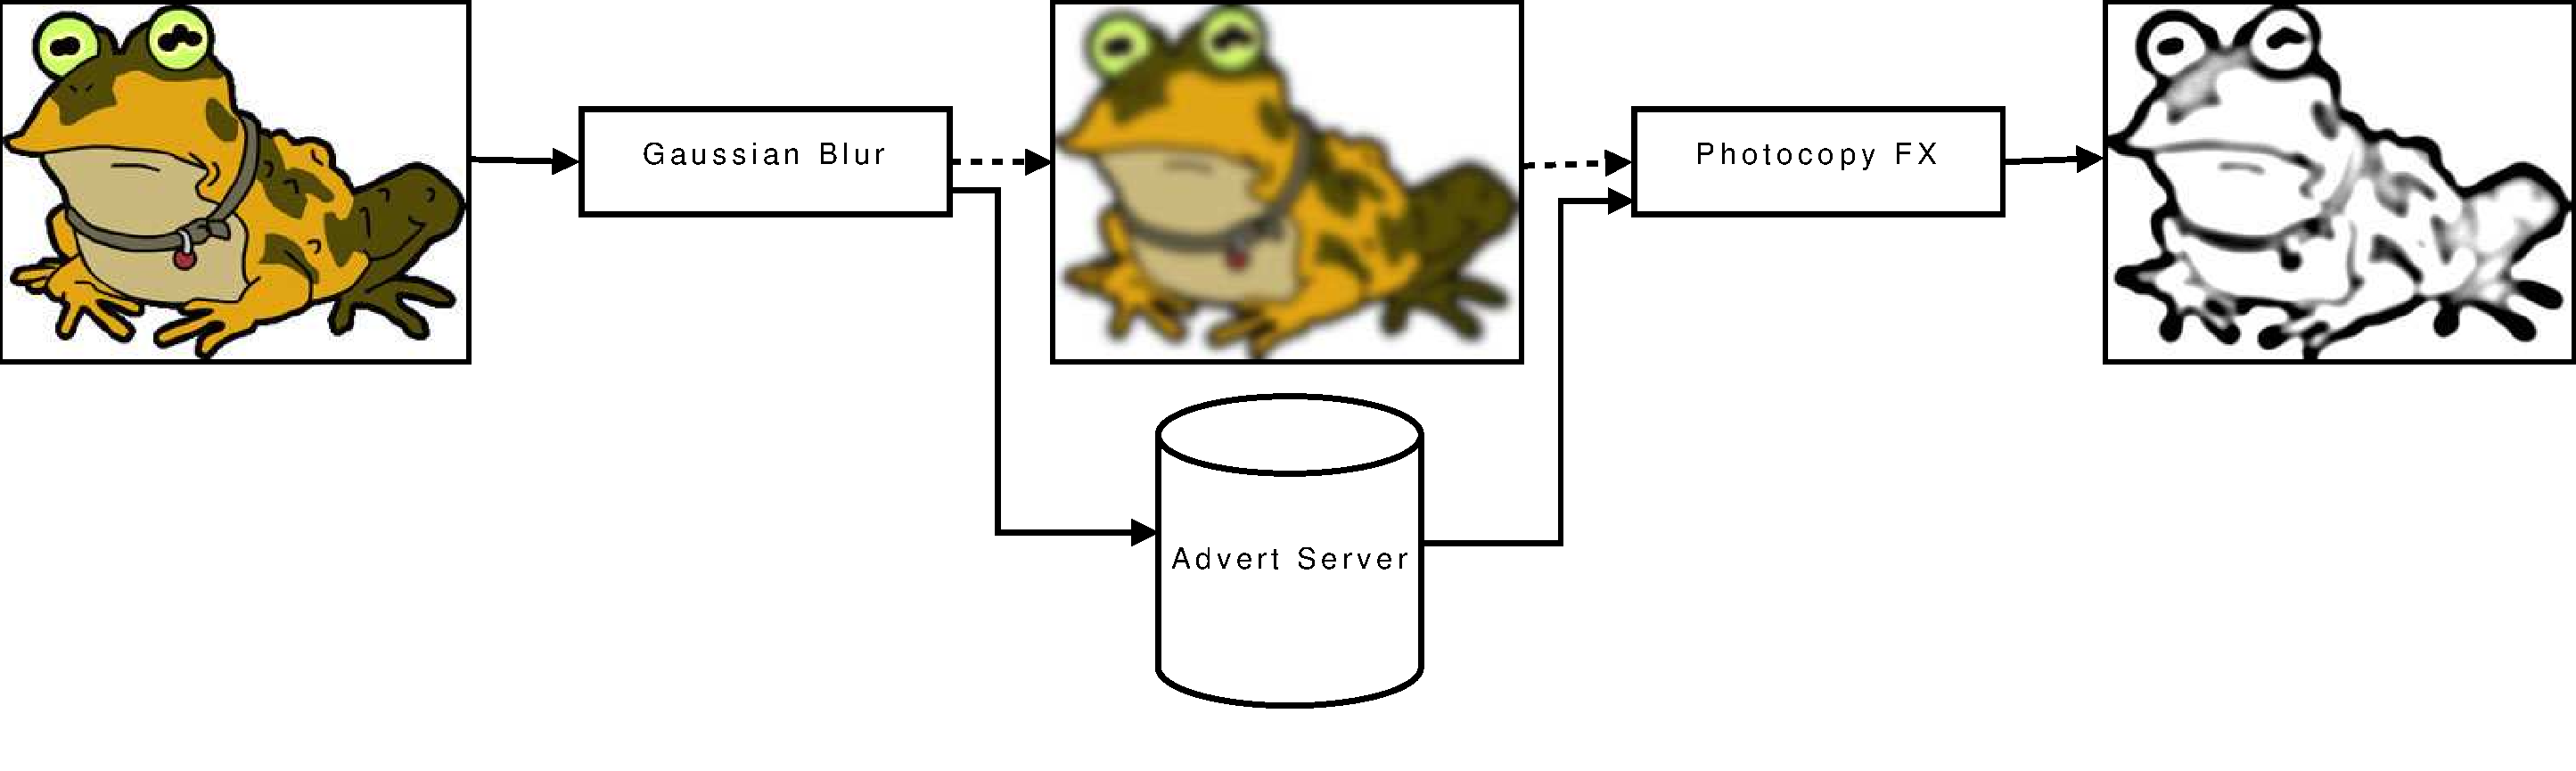
\includegraphics[width=14cm]{./figures/image_workflow.pdf} 
\caption{An Example of a Computational Workflow.\label{img-workflow}}
\end{center}
\end{figure*}

As far as we know, the Google App Engine has not been used as an application
storage server. Obviously, Google did not intend the App Engine to be used for
such purposes, hence the lack of spawning new processes or threads, or the
limited response time of a request. The most usable feature to us is the
distributed datastore, which could serve well as application storage
server (for Ibis). 

As an example for our application storage service, we took a closer look at
the \emph{JavaGAT AdvertService} \cite{javagat-www}. This provided us with main
functionality for our own Advert server, for adding, getting, deleting, and
finding objects in the Google datastore. Secondly we wrote a client library in
the Java programming language, which communicates over HTTP with the Advert
server, running at Google. Other Java programs can now use the client library
to store and retrieve (binary) application data at the Google App Engine.

In addition to this server, we wrote a Java client to communicate to the
server over HTTP(S), as can be seen from Figure \ref{introduction-overview}.
Once this library is imported into Ibis, Ibis applications can use the
library to store their data items in the data store.

\begin{figure*}[ht] %[placement] where placement is h,t,b,p
\begin{center}
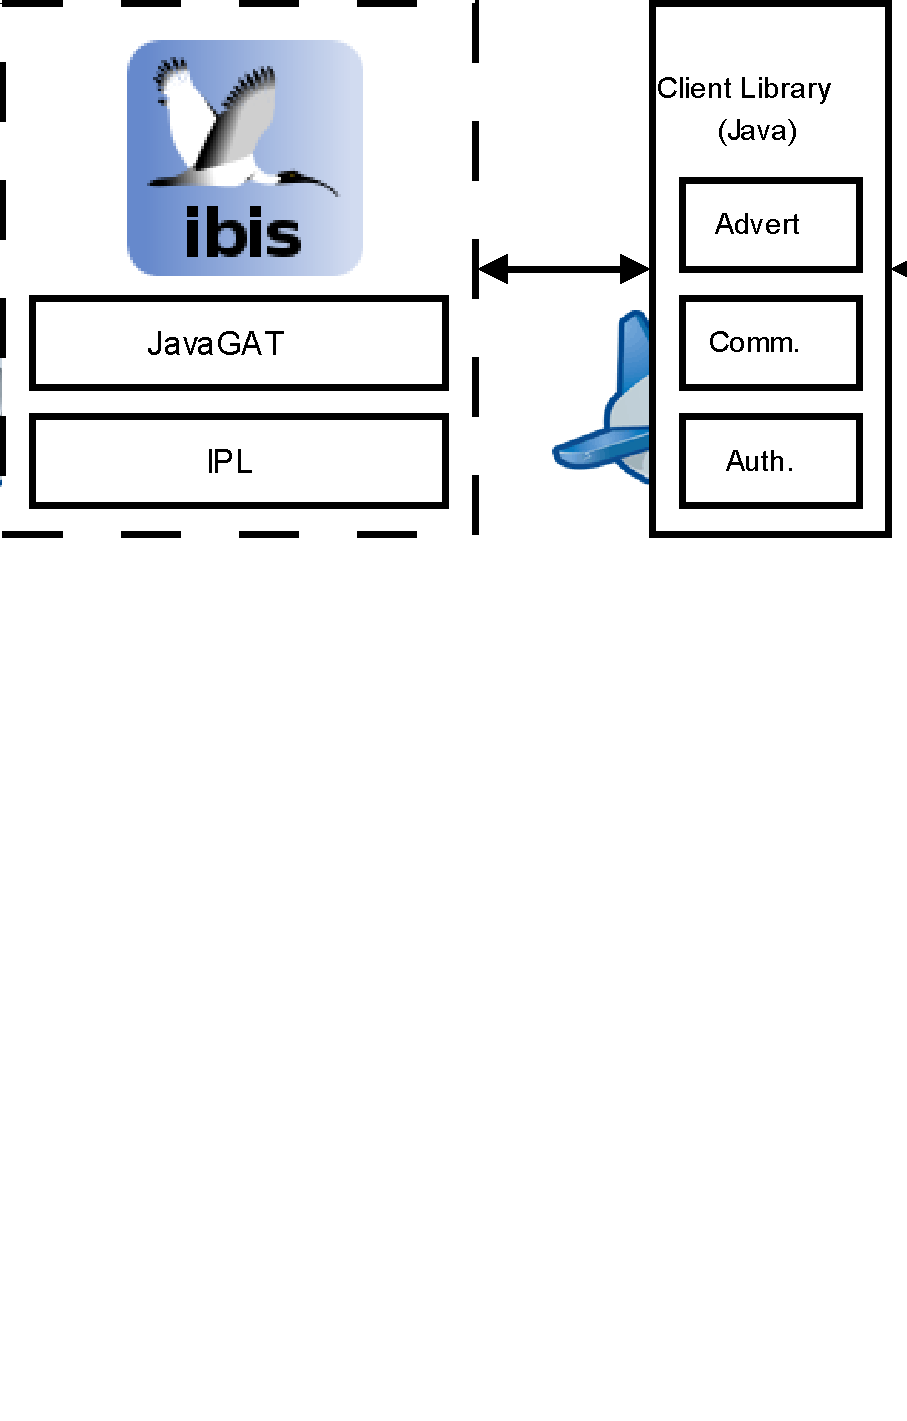
\includegraphics[width=14cm]{./figures/project_design.pdf} 
\caption{An Overview of our Project.\label{introduction-overview}}
\end{center}
\end{figure*}

As a result from building our Advert server similar to JavaGAT's AdvertService,
we could easily implement a JavaGAT AdvertService \emph{adaptor} for our
Google App Engine Advert server. Also we implemented a \emph{IPL server
bootstrap mechanism} for Ibis \cite{ipl-www}, where IPL servers can register
themselves in order to be found by other Ibis applications.

The rest of this paper is organized as follows. In Section \ref{related}
we look at related work, concerning \emph{Ibis} and the Google App Engine. In
Sections \ref{serverdesign} and \ref{serverimpl} we describe our Advert server
design and implementation, respectively, followed by the implementation of our
Advert client library in Section \ref{clientimpl}. Next we look at two
applications of Ibis in Section \ref{applications}. Finally we
present our benchmark results in Section \ref{benchmarks}, followed by our
conclusion and future work (Section \ref{conclusion}).
\newpage

%App Engine
\section{The App Engine}
\label{appengine}
April 7, 2008 Google launched a free-of-charge cloud computing service called
the \emph{Google App Engine}. Google offers a platform for developing and
hosting web applications at Google's data centers. Google virtualizes
applications and distributes databases across multiple servers and data centers.

\subsection{The Runtime Environment}
As of April 8th 2009 \cite{app-engine-java} the Google App Engine provides two
programming languages to build and run web applications. Besides \emph{Python}
\cite{python-www}, also the \emph{Java} \cite{java-www} programming language is
featured to develop web applications and run them on Google's resources. Since
the feature of running your applications in Java is still relatively new, we
focused on the Python runtime environment for scientific purposes.

A Python web application interacts with the App Engine web server using the CGI
protocol. An application can use a WSGI-compatible web application framework
using a CGI adapter. App Engine includes a simple web application framework,
called \emph{webapp}, to make it easy to get started. For larger applications,
mature third-party frameworks, such as \emph{Django} \cite{django-www}, work
well with App Engine.

The App Engine currently only supports Python 2.5.3. The Python interpreter runs
in a secured \emph{sandbox} environment to isolate our application for service
and security. The interpreter can run any Python code, including Python modules we
want to  include with our application, as well as the Python standard library.
The interpreter cannot load Python modules with C code; it is a `pure' Python
environment \cite{app-engine-sandbox}.

In addition, Google also provides a distributed database, called the
\emph{datastore}. The datastore provides robust scalable data storage for our
application. The datastore is designed with web applications in mind, and
emphasizes on read and query performance. It stores data entities with
properties, organized by application-defined kinds. It can perform queries over entities of
the same kind, with filters and sort orders on property values and keys. All
queries are pre-indexed for fast results over very large data sets. The datastore
supports transactional updates, using entity groupings defined by the application
as the unit of transactionality in the distributed data network
\cite{app-engine-datastore}.

\subsection{Limitations}
Although the Google App Engine provides us with resources, it also has some
limitations we should consider. All applications hosted on the App Engine
servers, are run within a sandbox. Spawning new processes using \texttt{fork()}
or threads are not allowed. Application code only runs in response to a web
request, and must return response data within thirty seconds. After the response
is sent, no code execution can take place.

An application can only access other computers on the Internet through the
provided URL fetch and email services and APIs. No socket connections to other
machines can be made. Other computers can only connect to the application by
making HTTP (or HTTPS) requests on the standard ports.

An application cannot write to the file system. An app can read files, but only
files uploaded with the application code. The app must use the App Engine
datastore for all data that persists between requests.

\subsection{Quotas}
\label{appengine-quotas}
The Google App Engine is free of use up to a certain level of used resources,
after which fees are charged for additional storage, bandwidth or CPU cycles
required by the application. As of June 29th, 2009, quotas that are enforced by
Google are provided in Figure \ref{quota-table}. Note that the table below some
quotas are billable, if the user provides payment information using \emph{Google
Checkout} \cite{google-checkout-www}. When you enable billing for your app, the
app's fixed quotas increase and an optional maximum can be set by the
application's administrator (the latter are called \emph{billable quotas})
\cite{app-engine-quotas}.

\begin{figure}[h,t]
\begin{center}
\begin{tabular}{| l | l | l | }
\hline
\multirow{2}{*}{Resource (*=billable)} & \multicolumn{2}{|l|}{Free Default
Quota} \\
\cline{2-3}
& Daily Limit & Maximum Rate \\
\hline
Requests & 1,300,000 requests & 7,400 requests/minute \\
\hline
Outgoing Bandwidth* & 1 gigabyte & 56 megabytes/minute \\ 
\hline
Incoming Bandwidth* & 1 gigabyte & 56 megabytes/minute \\
\hline
CPU Time* & 6.5 CPU-hours & 15 CPU-minute/minute \\
\hline
Datastore API Calls & 10,000,000 calls & 57,000 calls/minute \\
\hline
Stored Data* & 1 gigabyte & None \\
\hline
\end{tabular}
\caption{Google App Engine Free Default Quotas. \label{quota-table}}
\end{center}
\end{figure}

Note that Google has the right and ability to change these quotas over time.
During the development of our project, this has happened several times, both
increasing and decreasing quotas.

\subsection{Monitoring}
For the administrativor to monitor the quota already used by other users, one can
login to the administration panel. All quotas as described above can be monitored
from this website, and additionally, one can see when quotas will be reset (being
midnight, Pacific time\footnote{Historical note: The 24-hour replenishment cycle
was introduced in December 2008. It replaced a more complicated system of
`continuous' replenishment, to make it easier to report and control resource
usage.}).  Besides the monitoring of quotas, also various logs are available
(e.g. error logs, debug logs, and access logs), and one can check the contents of
the datastore as well. For more information on the administration panel, we
suggest reading \cite{app-engine-admin}.

\subsection{Scientific Purposes}
As far as we know, the Google App Engine has not been used for scientific
purposes, other than web services. Obviously, Google did not intend the App
Engine to be used for such purposes, hence the lack of spawning new processes
or threads, or the limited response time of a request. The most usable feature
to us is the distributed datastore, which could serve well as
\texttt{application storage server}, as will be described in more detail below.
\newpage

%Server Design
\section{Server Design}
\label{serverdesign}
Below we will describe some high-level design decisions we made, prior to
implementing our server on the Google App Engine.

\subsection{Server Structure}
\label{server-design-structure}
The server will have an iterative structure and servers clients on a
one-thread-per-client basis; it will receive a client request, process it and
return a reply (all in HTTP as described below). Since the App Engine distributes
each request to possibly a different server, concurrency can occur, so a form of
synchronization is needed. 

The datastore uses \emph{optimistic locking}\footnote{Optimistic locking (also
known as optimistic concurrency control) is based on the assumption that most
database transactions don't conflict with other transactions.} for concurrency
control. An update of an entity occurs in a transaction that is retried a fixed
number of times if other processes are trying to update the same entity
simultaneously. Our application can execute multiple datastore operations in a
single transaction, which either all succeed or all fail, ensuring the integrity
of data. 

Google provides us with an \emph{SQL} (Structured Query Language) alternative,
called the \emph{Google Query Language} (GQL). An example GQL query is shown in
figure \ref{gql-example}. These queries are rather powerful when using functions
like find(), as described below. Also, some security issues are triggered using
the GQL. Those are described in Section \ref{server-design-security}.

\begin{figure*}[ht] %[placement] where placement is h,t,b,p
\begin{center}
\begin{code}
db.GqlQuery("SELECT * FROM MyModel WHERE s1 >= :1 AND s2 < :2", "foo", "bar")
\end{code}
\caption{GQL Query example.\label{gql-example}}
\end{center}
\end{figure*}

\subsection{Client Functions}
The server provides some generic functions as an interface to its clients. These
functions adhere to the javadoc of the \emph{JavaGAT}\cite{javagat-www} (for
now). Below we will describe how these functions would be implemented. 

\subsubsection{HTTP Requests}
The Google App Engine only offers functions in a sandbox, as stated above. It is
not possible to make connections to the App Engine, other than using HTTP or
HTTPS. Furthermore, once a HTTP request is issued, a response is expected within
a few seconds, otherwise the connection times out. There is no specification on
the maximum size of an HTTP request/response.

Google offers an URL Fetch function, which supports five HTTP methods: GET, POST,
HEAD, PUT and DELETE. For the functions described below, it would be useful to
have an HTTP method that would allow us to send some (binary) data (i.e. POST or
GET), after which we do not only get a success return value; but also data as a
return value. This would be especially useful for the \texttt{find()} function.
The HTTP POST function servers our needs best, since the GET function translates
all data into a URL formatted String (which would be inappropriate for binary
data). Secondly, according to the HTTP RFC , the default HTTP response is a
status line (e.g. ``200 OK''), followed by a message body. This suits the needs
for the implementation of our server.

Our Java Adaptors could easily use these methods to authenticate themselves (with
or without Google Accounts), and call functions, possible sending data as
parameter of a function (using \emph{SOAP}\footnote{SOAP stands for Simple
Object Access Protocol, a protocol specification for exchanging structured
information in the implementation of Web Services. \cite{soap-www}} or
\emph{JSON} (JavaScript Object Notation) \cite{json-www} for example).

For Python \emph{simplejson} \cite{simplejson-www} is available, which is a
simple, fast, complete, correct and extensible JSON encoder and decoder for
Python 2.4+. It is pure Python code with no dependencies, but includes an
optional C extension for a serious speed boost. From Python 2.6, JSON is
contained in the standard library, but since Google makes use of Python version
2.5.2, it is likely that simplejson is needed.

\subsubsection{Functions to Implement} 
Looking at the javadoc of the JavaGAT \cite{javagat-javadoc}(the AdvertService in
specific), there are some basic functions we can implement using the App Engine.
First of all a very important function is the function called
\texttt{marshall()}, which takes a random object (stream of bytes) and creates a
String representation of this object. This object can then be used by the
following functions:

\begin{itemize}
\item \texttt{void add(MetaData, Object)}; Add an object with meta data to the
datastore
\item \texttt{void delete(path)}; Delete an object from the datastore
\item \texttt{String[] find(MetaData)}; Query the service for entries matching
a specified set of meta data
\item \texttt{Object getInstance(path)}; Gets an object from the datastore
\item \texttt{MetaData getMetaData(path)}; Gets meta data from the datastore
\item \texttt{String getPWD()}; Returns the current element of the name space
used
\item \texttt{void setPWD(path)}; Specify the element of the name space to be
used as reference for relative paths
\item \texttt{void exportDataBase(target URI)}; Imports the advert database
from persistent memory located at the given URI
\item \texttt{void importDataBase(source URI)}; Exports the advert database to
persistent memory located at the given URI 
\end{itemize}

Note that these functions are specific to the JavaGAT AdvertService, but could
also be used for the \emph{IPL Registry Bootstrap} service (see section
\ref{ipl}, and possibly could be placed somewhere in an Ibis library for general
use.

A good example are the \texttt{getPWD()} and \texttt{setPWD()} functions. Both
functions are necessary to make the AdvertService adapter for the Google App
Engine. However, these functions won't be very helpful for the other uses of our
service. That's why they won't be implemented into our library (which
communicates with the App Engine), but they will be in the adapter (locally).

\subsection{MetaData}
With the above in mind we also have to specify the MetaData object for other
services. Generally, a MetaData object consists of a number of key value tuples,
where both the keys and the values are Strings. A MetaData object should contain
some basic functionality:

\begin{itemize}
\item \texttt{String get(key)}; Gets the value associated to the provided key.
\item \texttt{String getData(int)}; Gets the value associated to the key retrieved by getKey(int).
\item \texttt{String getKey(int)}; Gets the i-th key of the MetaData.
\item \texttt{boolean match(MetaData)}; Match two MetaData objects.
\item \texttt{void put(key, value)}; Put an entry in the MetaData object.
\item \texttt{String remove(key)}; Removes an entry specified by the provided key.
\item \texttt{int size()}; Returns the number of entries in the MetaData.
\end{itemize}

Furthermore, the MetaData object implements \texttt{Serializable}, which means
the object can be converted into a sequence of bits so that it can be stored.

\subsection{Datastore Layout}
The App Engine scalable datastore stores and performs queries over data objects,
known as entities. An entity has one or more properties, named values of one of
several supported data types. A property can be a reference to another entity, to
create one-to-many or many-to-many relationships.

\subsubsection{Data Types Needed}
As we look at the javadoc from the AdvertService, we notice that we need to store
Advertisable objects in the Google Datastore, which is basically a key-value
pair. The client requests to store a sequence of bytes, which is marshaled by the
server and stored in the datastore.

The keys could be stored as a String, for example (as can be seen in the javadoc
of advert.MetaData). It would be nice to implement some sort of hierarchy for the
keys, if we consider that the server application could also be used as a
bootstrap server for the IPL registry. This could be implemented by the ``Key'',
provided by the Google Datastore.

The values are best stored as a string of bytes, since the client is allowed to
store any object in the datastore as wished. Google provides a data type for
these kind of data, which is called the BlobProperty . Blob is for binary data,
such as images. It takes a String value, but this value is stored as a byte
string and is not encoded as text, which is exactly what we need.

\subsubsection{Datastore Functions}
Besides traditional functions that Google provides to manipulate the datastore
(provided by the data modeling API, defined in \texttt{google.appengine.ext.db});
Google also provides an SQL like way to communicate with the datastore, called
the GQL.

\subsubsection{Garbage Collection}
Since the capacity of the datastore is limited to 500MB, we need some sort of
\emph{garbage collection} to keep our service usable for storing new data. This
is only possible by overwriting old data with new data (i.e. removing non-used
items to make room for new data). Removing old items is called garbage
collection.

\paragraph{TTL}
Initially we could give every data item stored in the server a Time to live
(TTL). This TTL could have a fixed value (for example 10 days), after which the
data will be removed from the datastore, making room for new data. Alternatively,
we could give data items a dynamic value for their TTL, depending on the usage of
the datastore (i.e. if the datastore is almost full, we will give data a shorter
TTL).

On every request (or once every x requests), we could query the datastore for
expired items and delete them from the datastore accordingly. Another option
would be that we remove the items which are expired as soon as we run out of free
storage space. This would give less overhead than starting a garbage collector
every request.

\paragraph{FIFO and LRU}
Secondly, if we would not give a TTL value to each data item stored in the
datastore, we could remove the oldest item as soon as we run out of free storage
space. By giving all items a timestamp as soon as we store then in the datastore,
we could find the oldest and remove it from the datastore to make room for new
data. Also we could make something like a LRU list (Least Recently Used), after
which we update the timestamp as soon as a data item was referenced or edited.
This way, only the data items that are least referenced are deleted, as soon as
we run out of storage.

\paragraph{Our Solution}
For now we would like to guarantee that a data item at least exists for a fixed
time span in the datastore. This way we prevent data items of being removed from
the datastore too quickly. Secondly the TTL should not be updated if a data item
is referenced. This could lead to clients referencing them only the keep them
alive in the datastore. Our main purpose for the TTL is to prevent clients from
storing data in the datastore and forgetting to delete it (which results in an
overfull datastore). Finally we won't need garbage collection every request, but
only when the datastore is reaching its limit (e.g. when 90\% is used). When the
datastore is full and there is no data to be evicted, we return an error to the
client, which throws an \texttt{AppEngineResourcesException}. The client can then
try again at a later moment in time, or use another server.

\subsection{Authentication and Privacy}
Google provides two forms of authentication with its App Engine.

\begin{itemize} 
\item By means of a Google Accounts (also used for Gmail, iGoogle, etc)
\item Google Apps for your Domain
\end{itemize}

For the first option, Google's unified sign-in system is used. All a user needs
is a valid email address (it doesn't need to be a Gmail address!) to sign up for
a Google Account. For the second option, users of Google Apps for your Domain can
choose to restrict all or part of their web application to only those people who
have a valid email address on their domain.

\subsubsection{Authentication through Google Accounts}
For our purposes it would be most attractive to make use of the authentication
through Google Accounts. An application can redirect a user to a Google Accounts
page to sign in or register for an account, or sign out; using simple functions
like \texttt{create\_login\_url()}. After a successful login session the
application can retrieve a User object to authenticate a user.

If one is to log in manually (\texttt{create\_login\_url()} was called), one
would see a login page, similar to that of other Google services, like Gmail for
example. Once one has pushed the `Sign in' button, username and password are sent
over HTTPS, after which a cookie is stored at the user side, containing a session
ID (ACSID). This cookie is used for all sessions until logout is initiated.
 
Note that this function is not very useful for our client, so we will have to
program the login process ourselves. There are solutions to interact with Google
data services, using cURL  for example .

\subsubsection{Own Authentication Scheme}
Second possibility would be to drop the concept of Google Account authentication,
and write our own authentication scheme (for example using a private-public key
pair). This has the advantage that we could apply a much more sophisticated
authentication scheme and give more guarantees with respect to the issues stated
above. A disadvantage is that it takes a lot more time and knowledge to implement
your own authentication scheme, while there is a perfectly fine solution at hand
(i.e. Google Accounts).

Another way of not using the authentication through Google accounts would be to
use the Django  framework, which is also supported by the Google Apps Engine.
Various examples of this authentication scheme exist.

\subsubsection{Server Authentication}
Both authentication schemes give us two options for server setups.

\begin{itemize}
  \item \textbf{Everyone Runs Its Own Service}; This way one could only
  authenticate himself by using a Google Account (i.e. one Google Account per
  organization), or restrict the application for only the domain of the
  organization using this service, or even to oneself. This way one would run out
  of resources less quickly than if one would use a (global) public service.
  Also, it is more reliable than using a public service; there is less chance of
  people reading and/or editing data stored by the service.
  \item \textbf{One Public Service for Everyone}; This way we would run an open
  service, accessible for everyone, without the need for a Google Account to
  authenticate oneself. A possible downside of this is that everyone can
  read/edit everyone's information. Also global public use might make the service
  run out of resources fast. Thus, for one global public service we can't give
  many guarantees.
\end{itemize}

\subsubsection{Conclusion}
Note that both solutions do not necessarily implement hierarchy in users. There
will be an interface for the administrator, but that stands aside of the service
we are offering (this interface is offered by the Google App Engine). Otherwise
it seems logical to use the Google Accounts for authentication (if we want to run
a 'private' service). For now we will implement two different servers; one
without any form of authentication (i.e. a public server), and one with
authentication (i.e. only the owner is able to use it, and additional users can
be added after the server is deployed).

\subsection{Security}
\label{server-design-security}
Finally we should take a look at security besides user authentication. More
decisions should be made as described below.

\subsubsection{(In)Secure Connections}
Google provides the means of having both insecure connections (HTTP, port 80), as
having secure connections (HTTPS, port 443). Naturally some data we would rather
not share in the open (for example passwords), so that would be a use for HTTPS.
The question is, if it would be wise (and necessary) to run all traffic over
HTTPS. We have to keep in mind that our bandwidth for HTTPS is limited (five
times less than our HTTP bandwidth), but is still a reasonable amount (see
Section \ref{appengine-quotas}). Plus we don't give any guarantees. If we run
out of HTTPS, we just have to wait another 24 hours and it will work again. Either way
configuration is done beforehand , when it comes to secure connections.

\subsubsection{GQL Queries}
SQL queries are generally vulnerable to SQL injection,
which is a technique that exploits a security vulnerability occurring in the
database layer of an application. Basically it would make it possible to insert
an SQL statement within a statement, and execute custom code. Usually this
custom code exists of malicious statements like \texttt{DROP}. Since the Google
App Engine's GQL Syntax only supports the \texttt{SELECT} stament, we do not
have to prevent this (see Figure \ref{gql-syntax}).

\begin{figure*}[ht] %[placement] where placement is h,t,b,p
\begin{center}
\begin{code}
  SELECT * FROM <kind>
    [WHERE <condition> [AND <condition> ...]]
    [ORDER BY <property> [ASC | DESC] [, <property> [ASC | DESC] ...]]
    [LIMIT [<offset>,]<count>]
    [OFFSET <offset>]

  <condition> := <property> {< | <= | > | >= | = | != } <value>
  <condition> := <property> IN <list>
  <condition> := ANCESTOR IS <entity or key>
\end{code}
\caption{GQL Syntax.\label{gql-syntax}}
\end{center}
\end{figure*}

In addition, the App Engine does not support multiple queries seperated by a
semi-colon (``\texttt{;}''), because it raises a parse error. Only one query at
a time can be executed and there is no support for nested queries also.

\newpage

%Server Implementation
\section{Advert Server Implementation}
\label{serverimpl}
Below we describe our (advert) server in more detail.

\subsection{User Authentication}
As described in the Server Design we will implement two servers, one without user
authentication (i.e. a public server without any guarantees), and a server which
requires authentication through Google Accounts.

\subsubsection{Google Accounts}
The most basic and obvious way to achieve authentication is single user
authentication (through Google Accounts). Basically only the owner is allowed to
use the advert service. According to the documentation provided by Google, there
is no variable that indicates if a user is owner of the application. Nonetheless
there is another function called \texttt{is\_current\_user\_admin()}, which is
available in the \texttt{google.appengine.api.users} package. By default the
owner of the application is administrator, and additional administrators can be
added through the administration panel. This fits our needs perfectly.

Once a client logged in through the Google login procedure (e.g. a Google login
page), the request handler at the server returns a user object, as shown in
Figure \ref{serverimpl-auth}. This object can then be used to identify a
user.

\begin{figure*}[ht] %[placement] where placement is h,t,b,p
\begin{center}
\begin{code}
user   = users.get_current_user()

if not user:
    self.error(403)
    self.response.headers['Content-Type'] = 'text/plain'
    self.response.out.write('Not Authenticated')
    return

if not users.is_current_user_admin():
    self.error(403)
    self.response.headers['Content-Type'] = 'text/plain'
    self.response.out.write('No Administrator')
    return
    
...
\end{code}
\caption{Authenticating a User.\label{serverimpl-auth}}
\end{center}
\end{figure*}

Other functions included in the \texttt{google.appengine.api.users} package are:

\begin{itemize} 
\item \texttt{create\_login\_url(dest\_url)}; which returns a URL that, when
visited, will prompt the user to sign in using a Google account, then redirect
the user back to the URL given as \texttt{dest\_url}.
\item \texttt{create\_logout\_url(dest\_url)}; which returns a URL that, when
visited, will sign the user out, then redirect the user back to the URL given as
\texttt{dest\_url}.
\end{itemize}

\subsection{The Datastore}
\subsubsection{Datastore Layout}
The Google App Engine datastore is not like a traditional relational database.
Data objects, or ``entities'', have a kind and a set of properties. For our
server we need a set of different data objects to store in our datastore.

\paragraph{(Advert) Objects}
Obviously, the main purpose of our server is to store binary (advert) objects.
For this purpose we designed the following entity to represent our advert data
(Figure \ref{serverimpl-ds}). First of all we will store a path, which will be
used for reference of a unique object (i.e. a key), which will be structured as a
directory structure. Secondly, we will store the author's name, for legal issues.
Next is the actual Advert object, which is stored as binary data. Finally we add
a TTL as will be discussed below.

\begin{figure*}[ht] %[placement] where placement is h,t,b,p
\begin{center}
\begin{code}
class Advert(db.Model):
  path   = db.StringProperty()
  author = db.UserProperty()
  ttl    = db.DateTimeProperty(auto_now_add=True)
  object = db.BlobProperty()
  
class MetaData(db.Model):
  path   = db.StringProperty()
  keystr = db.StringProperty()
  value  = db.StringProperty()
\end{code}
\caption{An Advert Object.\label{serverimpl-ds}}
\end{center}
\end{figure*}

Note that an Advert object can be \texttt{null}. Although we do not see why
just storing meta data would be useful, we do allow to store a \texttt{null}
object.

\paragraph{MetaData}
At our server, we would like to store meta data not as a binary object, but as
readable strings of data. This way, we can search meta data when it is queried.
According to the AdvertService API, a MetaData object should look like Figure
\ref{serverimpl-ds}. In this object, we just need to store key-value pairs, which
are String properties. Every object will be linked to a parent (Advert object),
as soon as it's created. Note that there is redundant information inside this
object, being the \texttt{path} value. We did this to simplify our GQL queries as
described in Section \ref{serverimpl-findmd}.

Just like the Advert object, a MetaData object can be null (i.e. no MetaData
is to be stored). The only way the object can then be referenced is by using
the specified pathname. 

\subsubsection{Transactions}
\label{serverimpl-trans}
Since the (Advert) object and the MetaData object are stored sequentially, it is
essential that they are stored either both, or neither of them, to ensure
consistency. Fortunately, the Google App Engine datastore provides a mechanism
for ensuring both are stored or, if the datastore fails, nothing is stored.
Using transactions, we can call a function and maintain atomicity. All
functionality of the App Engine can be used inside a function that is called in
transaction, except for GQL functions.

Another prequisite of transactions is that all data operated on must be in the
same entity group (this includes retrieving entities by key, updating entities, and
deleting entities). Entity group relationships tell App Engine to store several
entities in the same part of the distributed network. When the application
creates an entity, it can assign another entity as the parent of the new entity,
using the parent argument in the Model constructor. Assigning a parent to a new
entity puts the new entity in the same entity group as the parent entity. This is
exactly what we do when storing an object with meta data attached to it (all
meta data which belongs to a certain object have the same parent, being the
object itself). Notice that each root entity belongs to a separate entity group,
so a single transaction cannot create or operate on more than one root entity. 

\begin{figure*}[ht] %[placement] where placement is h,t,b,p
\begin{center}
\begin{code}
try:
  db.run_in_transaction(store, json) 
except db.TransactionFailedError, message:
  logging.error(message)
  ...
\end{code}
\caption{Transactions.\label{serverimpl-transfun}}
\end{center}
\end{figure*}

A small example of how transactions work inside the App Engine is shown in Figure
\ref{serverimpl-transfun}. In this example we encapsulated the transaction
function \texttt{store}, with arguments \texttt{json}, into a \texttt{try},
\texttt{except} statement. If the transaction fails, the operation's effects are not
applied, and the datastore API raises an exception, which in turn is caught by
the \texttt{except} statement and an error message is attached. The transction
could fail due to a high rate of contention, with too many users trying
to modify an entity at the same time. Or an operation may fail due to the
application reaching a quota limit. Or there may be an internal error with the
datastore.

Note that to ensure consistency of the datastore, we will also use transactions
to remove objects from the datstore. Again this is done sequentially. If one
delete function would fail, we would end op with an inconsistent copy of the
datastore. Hence we will again use transactions for atomicity and thus
consistency.

\subsubsection{Path Encoding}
To have the AdvertService work properly, we need some path encoding to save
Advert objects in the datastore. The Google App Engine itself provides one
solution, because every entity in the datastore has a key. When the application
creates an entity, it can assign another entity as the parent of the new entity.
Assigning a parent to a new entity puts the new entity in the same entity group
as the parent entity. Every entity belongs to an entity group, a set of one or
more entities that can be manipulated in a single transaction. An entity without
a parent is a root entity. An entity that is a parent for another entity can also
have a parent. A chain of parent entities from an entity up to the root is the
path for the entity, and members of the path are the entity's ancestors. The
parent of an entity is defined when the entity is created, and cannot be changed
later. The downside of this solution is that we have to create empty MetaData
objects for path nodes that are empty.

Another option is to save our own paths, using a namespace that identifies a
path, something like the UNIX system does (e.g. \texttt{/home/bboterm/.}). The
advantage of this model is that it works exactly analogue to the JavaGAT
AdvertService. The disadvantage of this is that we have to parse our own
pathnames, and keep track of them by means of a non-existing mechanism (i.e.
something that we need to build ourselves). Since this is not a major obstacle,
we will stick with the second approach. Note that all pathnames are allowed at
the server side. They are just used as identifiers of objects, not actual paths.

\subsection{Public Server Functions}
Below we will list some of the major functions the advert server will offer to
the client. These functions will be used by, for example, the JavaGAT
AdvertService adaptor for the App Engine.

\subsubsection{Logging In}
Since we are using ClientLogin service (as described above) to authenticate
ourselves to the App Engine, we won't need a separate login page. Sending our
credentials (session IDs) to the Appe Engine should be enough to authenticate
ourselves. For every request, our server will use a small section of code, which
looks like the code segment stated in Figure \ref{serverimpl-login}, to
authenticate the user.

\begin{figure*}[ht] %[placement] where placement is h,t,b,p
\begin{center}
\begin{code}
class AnyClass(webapp.RequestHandler):
  def get(self):
    user = users.get_current_user()

    if user and users.is_current_user_admin():
      self.response.headers['Content-Type'] = 'text/plain'
      self.response.out.write('Hello, ' + user.nickname())
    else:
      self.response.http_status_message(401)
      self.response.out.write('Some error.')
\end{code}
\caption{A MetaData Object.\label{serverimpl-login}}
\end{center}
\end{figure*}
      
\subsubsection{Receiving and Storing Binary Data}
An important function of the Advert Service is to accept and store binary data.

\paragraph{Binary Data Only}
For accepting just binary data, we can receive the entire message body and write
it to a variable, which is stored in the datastore accordingly. A sample code of
this function is shown in the code segment of Figure \ref{serverimpl-download}.
The first line identifies the class, which is called by the RequestHandler
(depending on the given URL). The second line says that we are expecting a POST
request. Then, a new \texttt{Bin()} data model is created (which in our case only
contains a field \texttt{data = db.BlobProperty()}). Then we fetch the body and
put in a temporary variable, before we store it as a \texttt{db.BlobProperty()}in
the database by calling \texttt{bin.put()}.

\begin{figure*}[ht] %[placement] where placement is h,t,b,p
\begin{center}
\begin{code}
class Download(webapp.RequestHandler):
  def post(self):
    bin = Bin()
    uploaded_file = self.request.body
    bin.data = db.Blob(uploaded_file)
    bin.put()
    self.redirect('/')
\end{code}
\caption{Accepting Binary Data.\label{serverimpl-download}}
\end{center}
\end{figure*}
      
\paragraph{Combination of Binary Data and Strings}
Although meta data will be stored in a different class, we won't apply a
different function to store MetaData objects, for the simple reason that if one
of these transfers would fail, it could lead to inconsistencies (see Section
\ref{clientimpl-sending-both}).

When receiving our binary object as a combination of both binary data and
unicode Strings, it will be received as one stream of bytes (assuming we're not
using the multipart/formdata method of Section \ref{clientimpl-sending-both}.
This means that we will have to dismember the message ourselves, which is
not as straightforward as it seems. The Google App Engine currently only
supports Python 2.5, which does not support bytes or byte arrays for data
manipulation.

We still managed to extract data using string manipulation. Essentially when the
App Engine receives the entire body as shown in Figure \ref{serverimpl-download},
it is stored as a raw string (no encoding) before it is stored as BLOB in the
datastore. We made use of that raw string as shown in Figure
\ref{serverimpl-raw-string}. In this example, we receive the message body and
store it into the raw string called `bytes'. After this we read the first byte
(\texttt{bytes[0:4]}), we use \texttt{ord()} to make it an integer, knowing the
length of the data sent. After that we send our Content-Type headers and write
the rest of the body to the standard output.

\begin{figure*}[ht] %[placement] where placement is h,t,b,p
\begin{center}
\begin{code}
bytes = self.request.body
length = ord(bytes[0:4])
self.response.headers['Content-Type'] = "image/gif"
self.response.out.write(bytes[5:length])
\end{code}
\caption{Manipulating a Raw String.\label{serverimpl-raw-string}}
\end{center}
\end{figure*}

\paragraph{Simplejson}
\label{serverimpl-simplejson}
Instead of using our own representation of unicode Strings and binary data, we
could also use a JSON representation. Once a serial JSON array or object has
been sent (see Section \ref{clientimpl-sending-both}), we are able to load it
into a server-side JSON object and decode it according to Figure
\ref{serverimpl-json}. The \texttt{simplejson.loads()} function decodes a
serial JSON String representation into a JSON array, after which we can access
its array entries like a regular array. 

\begin{figure*}[ht] %[placement] where placement is h,t,b,p
\begin{center}
\begin{code}
body = self.request.body
json = simplejson.loads(body)
...
advert.path   = json[0] #extract path from message
advert.object = json[2] #extract (base64) object from message
...
for k in json[1].keys():
  ...
  metadata.keystr = k
  metadata.value  = json[1][k]
...
\end{code}
\caption{Decoding a JSON object.\label{serverimpl-json}}
\end{center}
\end{figure*}

The same goes for a JSON object. We can construct a for loop like shown in
Figure \ref{serverimpl-json}, by iterating through all the keys and retrieving
their key-value pairs.

For reasons mentioned in Section \ref{clientimpl-sending-both}, the object is
not send in binary, but in unicode String format. For this reason, we can't
store it as a \texttt{db.BlobProperty()}, since this property expects unencoded
binary data only. The only option is to use the \texttt{db.TextProperty()},
since it is not limited to 500 characters, like the \texttt{db.StringProperty()}
is.

Before storing the JSON object it is checked to be a valid JSON object, which
should adhere to the syntax shown in Figure \ref{serverimpl-json-syntax}.
Otherwise an error is returned and the object is not stored. Note that storing a
JSON object is done in an atomic transaction, as described in section
\ref{serverimpl-trans}.

\begin{figure*}[ht] %[placement] where placement is h,t,b,p
\begin{center}
\begin{code}
[ string , { string : string , string : string , ... } | null , string | null ]
\end{code}
\caption{Advert syntax of a JSON object.\label{serverimpl-json-syntax}}
\end{center}
\end{figure*}

\subsubsection{Storing Meta Data}
Since MetaData needs to be searchable at the server-side, we will have to extract
the key-value pairs from the POST request and store them in the datastore
accordingly. This will be done in the opposite way of sending them at the Client
side (see Section \ref{clientimpl-sending-both}).

As of yet, the Google App Engine does not support Tuples, or key-value pairs as a
data type. Therefore we created our own MetaData class as described above. Also,
this MetaData cannot be stored into a list, because lists only supports primary
data types like integer and string. For that matter, we add an ID to the
MetaData, which is a child of the binary object stored in the datastore.

Another option would be to maintain two lists of strings, where the indexes of
the lists link the key and the value of the MetaData. However, we are not sure of
those lists maintain order (which could mess up the MetaData).

Finally, we could also append all data in two strings and have them separated by
special delimiter. Downside of this method is that we could run out of the
maximum length of strings (which is 500 bytes).

Once data has been stored successfully, we send an HTTP 201 (Created) status
code, and return the TTL in the message body. If an entry already exists at the
specified path, that entry gets overwritten, and a warning is issued. This is
done by sending an HTTP 205 (Reset Content) Status Code and a warning in the
message body.

Note that if meta data is \texttt{null}, no meta data will be stored in the
datastore, since it would not make any sense to search for data that is never
sent.

\subsubsection{Finding MetaData}
\label{serverimpl-findmd}
When the MetaData has been stored in the datastore, we should be able to process
find() requests by clients. First a MetaData object is received, which is then
tried to be matched with MetaData already present in the datastore. For this
purpose we will use the GQL as described above.

To process the find() request, we have to check all the key-value pairs given
by the client and compare them to the key-value pairs of all MetaData objects
in the datastore. Since all key-value pairs are stored in one `table', we
have to group them by path, after which we can check all key-value pairs per
MetaData object.

Comparing the MetaData object sent by the user with the MetaData present in the
datastore can be achieved in two ways. One approach is to make a selection of
all paths available and check the key-value pairs on a per path basis. This
is done by the GQL query shown in Figure \ref{serverimpl-find}.

\begin{figure*}[ht] %[placement] where placement is h,t,b,p
\begin{center}
\begin{code}
query = db.GqlQuery("SELECT * FROM MetaData")

paths = Set()

for bin in query:
  paths.add(bin.path)
  
paths  = list(paths)
self.response.out.write(paths)

for path in paths[:]:
  for k in json.keys():
    query = db.GqlQuery("SELECT * FROM MetaData WHERE path = :1 AND keystr = :2
                         AND val = :3", path, k, json[k])
    if query.count() < 1:
      paths.remove(path)
      break

if len(paths) < 1:
  self.error(404)
  self.response.headers['Content-Type'] = 'text/plain'
  self.response.out.write('Not Found')
  return

self.response.out.write(simplejson.dumps(paths))  
\end{code}
\caption{Functionality of \texttt{find()} Function.\label{serverimpl-find}}
\end{center}
\end{figure*}

To obtain an array of all paths (without duplicates), we would usually use the
`DISTINCT' keyword from SQL. Since the GQL does not support the `DISTINCT'
keyword we have to make our own unique array of keys. We do this by using the
\texttt{Set()} data type, which maintains a unique set of paths (duplicates are
automatically overwritten).

After we have a distinct set of all paths, we iterate through the list and
match every key-value pair with the key-value pair given by the user. If one
pair does not match, we remove the path from the list, and start over
inspecting the next path in the list. Eventually we will have a list of paths
which contains all paths that meet all requirements given by the user. 

The return value of all metadata found is a String array, which again needs to be
formatted in such a way that it can be sent as one String. Obviously we will
use simplejson to do so. If no entry is found, we will send a 404 response
code, accompanied by the text `Not Found' in the message body.

A second option to implement the \texttt{find()} function would be to first
find all paths that meet the requirements given by the first key-value pair.
Then do the same for the second key-value pair and accordingly take the
intersection between the two search results. This process should be repeated
until all key-value pairs have been checked. The downside of this approach is
that there is no obvious method to perform the intersection between two search
results at the Google App Engine. This approach requires a \emph{for-loop} to
iterate through all items in the first search result and check them with the
second. 

\subsubsection{Returning an Object From the Datastore}
This function will send binary data back to client. Basically, this function only
sends an Object to the standard output (the HTTP connection), which looks like
Figure \ref{serverimpl-bin-response}. Of Course, we first need to fetch the
requested object from the datastore, which will be done using GQL Queries. 
%TODO: <more to follow>

\begin{figure*}[ht] %[placement] where placement is h,t,b,p
\begin{center}
\begin{code}
self.response.headers['Content-Type'] = "application/octet-stream"
self.response.out.write(bin.data)
\end{code}
\caption{HTTP Response with Binary Data.\label{serverimpl-bin-response}}
\end{center}
\end{figure*}

\subsubsection{Removing an Object From the Datastore}
To remove an (Advert) object from the datastore, a user calls the
\texttt{delete()} function, with a pathname as argument. Obviously, the most
straightforward way to remove an item from the datastore is to query all
objects and meta data that match the pathname given. Naturally, we want to
perform the removal of the object and associated meta data in transaction,
because we do not want inconsistencies in our datastore (i.e. querying meta
data of which the associated object does not exist anymore).

The only problem we have now is that we cannot perform queries inside a
transaction, since the Google App Engine does not allow us to do so. The
solution that Google provides is either to work with keys (which is not
feasible in our case), or prepare your queries before performing the
transaction. We adapted this solution by sending our query results to a
\texttt{remove()} function, which iterates through the query results and
deletes all objects and meta data given to the function.

\subsection{Private Server Functions}
Below we will describe some of the private server functions provided for the
advert service.

\subsubsection{Garbage Collector}
As described above, we will use some form of TTL to determine whether a data item
stored is still needed in the datastorage. When a data item is expired, it will
be removed automatically using a mechanism called the garbage collector.
The source code of our garbage collector can be found in Figure
\ref{serverimpl-gc}.

\begin{figure*}[ht] %[placement] where placement is h,t,b,p
\begin{center}
\begin{code}
def gc(): #garbage collector
  query = db.GqlQuery("SELECT * FROM Advert WHERE ttl < :1", 
                      datetime.datetime.today() + datetime.timedelta(days=-10))
  
  for advert in query: #all entities that can be deleted
    advert.delmd()     #delete all associated metadata
    advert.delete()    #delete the object itself
\end{code}
\caption{The Garbage Collector.\label{serverimpl-gc}}
\end{center}
\end{figure*}

By calling \texttt{gc()}, we activate our garbage collector, which, in turn,
executes a GQL query, selecting all data that has been added to the datastore
earlier than ten days ago. To achieve this we use the \texttt{timedelta()}
object, provided by the \texttt{datetime} class. A timedelta object
represents a duration, the difference between two dates or times, and is ideal
for our garbage collector.

The query results in an iterable list of advert objects that can be removed
from the datastore. We should not forget that also all the MetaData
associated with the Advert object should be removed alongside the object itself.
Therefore we wrote a function inside the advert class, called \texttt{delmd()},
that automatically deletes all its metadata. Once this is done, the object
itself is deleted and the garbage collection process is finished.


% \subsubsection{Data Matching}
% For our \texttt{find()} function, we will need some internal `match' function,
% which can query the database to see if the specified data item is present in the
% datastore. For this matching, we will have an internal function which is able to
% match data received from the client with data present in the datastore. 
% %TODO: <more to follow>



\newpage

%Client Implementation
\section{Client Library}
\label{clientimpl}
Now that we have designed and implemented our application storage server, it is
time to build a client library, which communicates to the application storage
server, in order to create transparency for the user. Our client library is
completely written in \emph{Java} \cite{java-www} and needs at least Java
version 1.5 to compile.

\subsection{Public Functions}
Similar to the public functions specified in the server design (Section
\ref{serverdesign-pub}), we specified our client library functions. These
functions are also very similar to the JavaGAT API, which we will explain
further in Section \ref{applications-advertservice}. The following public
functions are available:

\begin{itemize}
	\item \texttt{void add(MetaData, Object)} 
	\item \texttt{void delete(path)}
	\item \texttt{String[] find(MetaData)}
	\item \texttt{Object getInstance(path)}
	\item \texttt{MetaData getMetaData(path)}
	\item \texttt{String getPWD()}
	\item \texttt{void setPWD(path)} 
\end{itemize}

All functions do exactly as described in Section \ref{serverdesign-pub}. In
addition to the server's public functions, two functions have been added to the
Advert library, being the \texttt{getPWD()} and the \texttt{setPWD()}. This is
implemented if a user wishes to use relative paths in stead of absolute paths.

In addition, we also added two constructors. One is the default constructor,
which creates an empty \texttt{MetaData} object. The other is a constructor
which takes a serialized form as an argument and returns a \texttt{MetaData}
object with the serialized key-value pairs already inserted. The serialized
form needs to look like this: \texttt{key1=value1,key2=value2,key3=value3}.

\subsection{Data Types}
In addition to public functions, we also implemented an extra data type, called
\texttt{MetaData}. In essence this is for storing key-value pairs, just like
meta data is stored at the server. The only difference is that a
\texttt{MetaData} object has more functionality than just key-value pairs.

\begin{itemize}
	\item \texttt{String get(key)}; Gets the value associated to the provided key 
	\item \texttt{String getData(int)}; Gets the value associated to the key
		retrieved by \texttt{getKey(int)}
	\item \texttt{String getKey(int)}; Gets the \texttt{i}-th key of the
		\texttt{MetaData}
	\item \texttt{boolean match(MetaData)}; Match two \texttt{MetaData} objects 
	\item \texttt{void put(key, value)}; Put an entry in the \texttt{MetaData} object 
	\item \texttt{String remove(key)}; Removes an entry specified by the provided
		key
	\item \texttt{int size()}; Returns the number of entries in the \texttt{MetaData} 
\end{itemize}

As one can see, a significant number of user functions is added to the
\texttt{MetaData} object. A lot of functions adhere to the \texttt{MetaData}
object provided by the JavaGAT \emph{AdvertService}. We will look deeper into
this when we discuss the AdvertService in Section
\ref{applications-advertservice}.

\subsection{Transfer Protocol}
Below we will describe the transfer protocol in more detail, as from a client
point of view. All our communication is done by the \texttt{Communication}
class, which is called by the public functions stated above. 

First we will describe some basics of how Java manages HTTP connections. After
that, we will take a look at the actual protocol, which is stated in both the
server design and implementation.

\subsubsection{HTTP(S) Connections}
Since our client is implemented in pure Java, it is useful to make use of the
\texttt{java.net} class, which allows us to make HTTP connections to the
App Engine. By creating an URL object like shown in Figure \ref{clientimpl-url}.

\begin{figure*}[ht] %[placement] where placement is h,t,b,p
\begin{center}
\begin{code}
URL url = new URL("http://ibis-advert.appspot.com/");
HttpURLConnection httpc = (HttpURLConnection) url.openConnection();
\end{code}
\caption{Opening an HTTP Connection.\label{clientimpl-url}}
\end{center}
\end{figure*}

Now it is possible with the use of the various functions in both classes to get
all information needed; like status-codes, HTTP Headers, and the message body.
This we will discuss below when we talk about the HTTP response.

In addition to HTTP connections, it is also possible in Java to make HTTPS
connections. This is done automatically by the \texttt{HttpURLConnection}
class, when a URL with scheme \texttt{https://} is opened.

% however, this is not as straightforward as making HTTP connections.
% To make an HTTPS connection we will need to import the
% \texttt{java.security.Security} class (amongst others). In addition, if we look
% at Figure \ref{clientimpl-https}, we see that the code adds us to the
% \texttt{security.provider} list in \texttt{java.security}. After these lines of
% code we will be able to make an HTTPS connection just like we did with making
% HTTP connection above (i.e. \texttt{url.openConnection()}). All sample code is
% fully operational at our branch in the JavaGAT SVN Repository .
% 
% \begin{figure*}[ht] %[placement] where placement is h,t,b,p
% \begin{center}
% \begin{code}
% Security.addProvider(new com.sun.net.ssl.internal.ssl.Provider());
% 
% Properties properties = System.getProperties();
% 
% String handlers = System.getProperty("java.protocol.handler.pkgs");
% if (handlers == null) { //nothing specified yet (expected case)
%     properties.put("java.protocol.handler.pkgs",
%         "com.sun.net.ssl.internal.www.protocol");
% } 
% else { //something already there, put ourselves out front
%     properties.put("java.protocol.handler.pkgs",
%         "com.sun.net.ssl.internal.www.protocol|".concat(handlers));
% }
% System.setProperties(properties);
% \end{code}
% \caption{Setting up an HTTPS Connection.\label{clientimpl-https}}
% \end{center}
% \end{figure*}

\subsubsection{HTTP POST Method}
Secondly, it is of great importance to create an HTTP POST request for both
authentication and sending data to the App Engine. The simplest option is to send
a various number of URL encoded strings. An example of making such an HTTP POST
request can be seen in Figure \ref{clientimpl-post}. We enable sending output to
the connection just created, calling \texttt{urlc.setDoOutput(true);}. After
making this call we are able to open an OutputStreamWriter to which we can write
our POST data. Multiple fields are separated by an ampersand (`\texttt{\&}'),
and variable names and values are separated by the equal sign. In this example we
write the author's name and content to an HTTP POST request.

\begin{figure*}[ht] %[placement] where placement is h,t,b,p
\begin{center}
\begin{code}
/* Setting up POST environment. */
httpc.setRequestMethod("POST");
httpc.setDoOutput(true);
OutputStreamWriter out = new OutputStreamWriter(httpc.getOutputStream());

/* Writing POST data. */
out.write("author=bbn230&content=test");
out.close();
\end{code}
\caption{Making an HTTP POST request.\label{clientimpl-post}}
\end{center}
\end{figure*}

% \paragraph{Sending Binary Data}
% In addition to just making HTTP post requests, it is also possible to send binary
% data (commonly used for uploading files to web servers via HTTP). Again, this is
% a step more difficult. We have to make sure the server expects a binary string of
% data. This is shown in Figure \ref{clientimpl-binpost}. After the request has
% been made, the content can be extracted from the message body by the server and
% can be stored accordingly.
% 
% \begin{figure*}[ht] %[placement] where placement is h,t,b,p
% \begin{center}
% \begin{code}
% /* Setting up POST environment. */
% urlc.setDoOutput(true);
% urlc.setRequestProperty("Content-Type", "application/octet-stream");
% \end{code}
% \caption{Making a binary HTTP POST request.\label{clientimpl-binpost}}
% \end{center}
% \end{figure*}

\subsubsection{HTTP Response}
After the HTTP request is sent, we are able to receive the HTTP response. To
begin with, we will download the response headers sent by the web server, after
which we can retrieve the body.

\paragraph{Headers}
How to receive the headers of an HTTP response is shown in Figure
\ref{clientimpl-headers}. Already, by receiving the response code, we can
distinguish errors from successful requests. Response codes of the form 1xx
are informational and those of the form 2xx mean success. Response codes
of the form 3xx are used for redirection, and 4xx and 5xx are used for
errors (client and server respectively). For example: 200 stands for success, 403 for
authentication required, and 404 for not found.

\begin{figure*}[ht] %[placement] where placement is h,t,b,p
\begin{center}
\begin{code}
/* Retrieving headers. */
System.out.println(httpc.getResponseCode());
System.out.println(httpc.getRequestMethod());
for (int i = 0; httpc.getHeaderField(i) != null; i++) {
    System.out.println(httpc.getHeaderField(i));
}
\end{code}
\caption{Retrieving HTTP response headers.\label{clientimpl-headers}}
\end{center}
\end{figure*}

After checking the response code, we can retrieve additional headers. In our case
(using the App Engine as our web server), we have listed an example of receiving
a successful response (Figure \ref{clientimpl-200}). Again, a status header is
sent, followed by the server type, the date, and some other info. Note that
``Content-Length'' can be really useful to determine our buffer size in the next
step.

\begin{figure*}[ht] %[placement] where placement is h,t,b,p
\begin{center}
\begin{code}
HTTP/1.0 200 OK
Server: Development/1.0
Date: Wed, 11 Mar 2009 11:25:05 GMT
Cache-Control: no-cache
Content-Type: image/gif
Content-Length: 18006
\end{code}
\caption{Example of HTTP response headers.\label{clientimpl-200}}
\end{center}
\end{figure*}

\paragraph{Cookies}
\label{clientimpl-cookies}
A `special' type of HTTP header that can be retrieved from sending an HTTP
request are cookies. Just like all the other headers, it is retrieved with the
code stated above. When printed to screen, it will look similar to the request
shown in Figure \ref{clientimpl-cookies-resp}. This code above is taken from
retrieving the URL \url{http://www.google.nl/}. As you can see, this cookie
consists out of multiple parts, but would normally be stored as one cookie in your
browser. In this case, the cookies name is ``PREF'', and its content is
``ID=8f3c26(\ldots)zrigB6''. Finally it comes with an expiration time and date,
a path, and a domain. This information will be needed when we want to authenticate
ourselves to the App Engine.

\begin{figure*}[ht] %[placement] where placement is h,t,b,p
\begin{center}
\begin{code}
HTTP/1.1 200 OK
Cache-Control: private, max-age=0
Date: Wed, 11 Mar 2009 11:57:38 GMT
Expires: -1
Content-Type: text/html; charset=ISO-8859-1
Set-Cookie: 
  PREF=ID=8f3c262a9b38330e:TM=1236772658:LM=1236772658:S=L2ORt13rUlzrigB6; 
  expires=Fri, 11-Mar-2011 11:57:38 GMT; path=/; domain=.google.nl
Server: gws
\end{code}
\caption{An HTTP response including cookies.\label{clientimpl-cookies-resp}}
\end{center}
\end{figure*}

\paragraph{Message Body}
Once we have received all headers and parsed them accordingly, we are able to
get the actual body. As we can see from Figure \ref{clientimpl-body}, the most
important thing is getting the stream, provided by the \texttt{getInputStream()}
function. After we have done this, we can basically do anything with our
InputStream. In this case we print it to the console, but we could also save it
in a buffer and manipulate it, or write it do disk, etc. After we are done
receiving the InputStream, we close the InputStream, effectively closing the
connection.

\begin{figure*}[ht] %[placement] where placement is h,t,b,p
\begin{center}
\begin{code}
BufferedReader in = 
  new BufferedReader(new InputStreamReader(httpc.getInputStream()));
String inputLine;

while ((inputLine = in.readLine()) != null) {
    System.out.println(inputLine);
}
in.close();
\end{code}
\caption{Retrieving the HTTP response's body.\label{clientimpl-body}}
\end{center}
\end{figure*}

\subsubsection{Object Encoding}
\label{clientimpl-encoding}
As shown in our server design (Section \ref{serverdesign-encoding}), we are using
JSON for encoding our objects before sending them to the server. In our client
library, we make use of the \emph{Json-lib} library \cite{json-lib-www}, which
fully implements the JSON format. A simple examples is given in Figure
\ref{clientimpl-json}, where we transform a \texttt{MetaData} object into a
serialized JSON object.

\begin{figure*}[ht] %[placement] where placement is h,t,b,p
\begin{center}
\begin{code}
JSONObject    jsonobj = new JSONObject();
Iterator<String> itr  = metaData.getAllKeys().iterator();

while (itr.hasNext()) {
	String key   = itr.next();
	String value = metaData.get(key);
	jsonobj.put(key, value);
}

String serialForm = jsonobj.toString();
\end{code}
\caption{JSON Encoding in Java.\label{clientimpl-json}}
\end{center}
\end{figure*}

This serialized form can now be send to the server using the HTTP POST method,
as described above.

\subsection{Authentication and Privacy}
\label{clientimpl-auth}
Finally we will describe how authentication is done. All functionality which
concerns authentication is done in the \texttt{Authentication} class, present
in the Advert client library. Logging in is done through Google Accounts (as
can be seen from Sections \ref{serverdesign} and \ref{serverimpl}).

\subsubsection{Google Login Page}
We have looked at the login page of a typical App Engine application, and we
have stripped the unnecessary HTML from the login form. As we can see from the
result shown in Figure \ref{clientimpl-loginform}, the login form is quite
comprehensive. The login form has a lot of extra (hidden and redundant) fields,
which we did not expect to find.

\begin{figure*}[ht] %[placement] where placement is h,t,b,p
\begin{center}
\begin{code}
<form id="gaia_loginform" 
action="https://www.google.com/accounts/ServiceLoginAuth?service=ah
    &amp;sig=d71ef8b8d6150b23958ad03b3bf546b7" 
  method="post"
  onsubmit="return(gaia_onLoginSubmit());">

<input type="hidden" name="ltmpl" value="gm">
<input type="hidden" name="continue" id="continue"
  value="http:// bbn230.appspot.com/_ah/login?
  continue=http://bbn230.appspot.com/" />
<input type="hidden" name="service" id="service" value="ah" />
<input type="hidden" name="ltmpl" id="ltmpl" value="gm" />
<input type="hidden" name="ltmpl" id="ltmpl" value="gm" />
<input type="hidden" name="ahname" id="ahname" value="Personal" />
<input type="text" name="Email"  id="Email" size="18" value="" />
<input type="password" name="Passwd" id="Passwd" size="18" />
<input type="checkbox" name="PersistentCookie" id="PersistentCookie" 
  value="yes" />
<input type="hidden" name='rmShown' value="1" />
<input type="submit" class="gaia le button" name="signIn" value="Sign in" />
<input type="hidden" name="asts" id="asts" value="">
</form>
\end{code}
\caption{Stripped down version of the App Engine
login page.\label{clientimpl-loginform}}
\end{center}
\end{figure*}

We are not sure what all hidden fields do, and if they are really necessary, but
simulating this login page by posting all this would make our HTTP POST request
quite large.

\subsubsection{Google Account Authentication API}
An alternative for simulating the login page is the \emph{Account
Authentication API} \cite{account-auth-api}. The Account Authentication API
comes in two forms. One form for installed \emph{Google Apps}
\cite{google-apps-www}, which is called \emph{ClientLogin}, the other is for Web
Apps, and is called \emph{OAuth} or \emph{AuthSub}.

\paragraph{ClientLogin}
Typically, ClientLogin is used for Installed applications that need to access
Google services protected by a user's Google or Google Apps. To make use of this
API, we will make a HTTP POST request to
\url{https://www.google.com/accounts/ClientLogin}, to which we send our
credentials as shown in Figure \ref{clientimpl-clientlogin}.

\begin{figure*}[ht] %[placement] where placement is h,t,b,p
\begin{center}
\begin{code}
StringBuilder content = new StringBuilder();
content.append("Email=").append(URLEncoder.encode("jondoe@gmail.com", 
  "UTF-8"));
content.append("&Passwd=").append(URLEncoder.encode("north23AZ", "UTF-8"));
content.append("&service=").append(URLEncoder.encode("ah", "UTF-8"));
content.append("&source=").append(URLEncoder.encode("Google App Engine", 
  "UTF-8"));
\end{code}
\caption{Preparing our ClientLogin credentials.\label{clientimpl-clientlogin}}
\end{center}
\end{figure*}

We created a Google Account for testing purposes and made a successful connection
using that account. The response of the ClientLogin is shown in Figure
\ref{clientimpl-clientlogin-response}.

\begin{figure*}[ht] %[placement] where placement is h,t,b,p
\begin{center}
\begin{code}
HTTP/1.1 200 OK
Content-Type: text/plain
Cache-control: no-cache, no-store
Pragma: no-cache
Expires: Mon, 01-Jan-1990 00:00:00 GMT
Date: Mon, 16 Mar 2009 14:07:25 GMT
X-Content-Type-Options: nosniff
Content-Length: 497
Server: GFE/1.3
----
SID=DQA(...)bjG
LSID=DQA(...)nSV
Auth=DQA(...)ub4
\end{code}
\caption{A response from ClientLogin.\label{clientimpl-clientlogin-response}}
\end{center}
\end{figure*}

Currently, `SID' and `LSID' are not used by the \emph{Google API}, so we just
need to extract the `Auth' value. Usually this value can be used directly on a
service its API (when providing a developer key), but unfortunately, the Google
App Engine is not listed in the Google data API library \cite{service-api}.
There is a workaround for still being able to connect to the App Engine, by
connecting to a App Engine's login page like Figure \ref{clientimpl-aelogin}.
In this example, \texttt{Auth} is a variable that contains the token acquired
by the example of Figure \ref{clientimpl-clientlogin-response}. 

\begin{figure*}[ht] %[placement] where placement is h,t,b,p
\begin{center}
\begin{code}
url = new URL("http://bbn230.appspot.com/_ah/login?auth="+ Auth);
\end{code}
\caption{Logging In for a Session Cookie.\label{clientimpl-aelogin}}
\end{center}
\end{figure*}

Connecting to this page will return a cookie with a session ID, just like the
one described in Section \ref{clientimpl-cookies}, only with a token called
`ACSID', with which we can identify ourselves to the App Engine for every
subsequent request.

\paragraph{AuthSub}
Web applications that need to access services protected by a user's Google or
Google Apps (hosted) account can do so using the Authentication Proxy service. To
maintain a high level of security, the proxy interface, called AuthSub, enables
the web application to get access without ever handling their users' account
login information. Before using, verify that the Google service to be accessed
supports the Authentication service. Some Google services may allow access only
to web applications that are registered and use secure tokens. We have not tried
AuthSub to authenticate ourselves at the App Engine. We will not use it as our
primary authentication mechanism because if our users would want to install an
advert server, it would require extra effort, because they need to register
themselves first before this service can be used.

\subsubsection{Persistent Authentication}
Also, to maintain session with the server, we want to pass a session ID through
cookies. Also, this can be done through Java by setting the appropriate headers.
For example, if we want to send a cookie with the name ``SID'' and the content
``abcde'', we could code this in Java as shown in Figure
\ref{clientimpl-cookies-req}. This code will add the cookie to the HTTP request,
after which the response headers and body can be fetched.

\begin{figure*}[ht] %[placement] where placement is h,t,b,p
\begin{center}
\begin{code}
urlc.addRequestProperty("Cookie", "SID=abcde");
\end{code}
\caption{Sending cookies in Java.\label{clientimpl-cookies-req}}
\end{center}
\end{figure*}

Because the authentication cookies, as provided by the Google App Engine,
generally expire after 24\,hours. This means that, unless the user restarts the
Advert library, the user will receive an \emph{HTTP 403 Authentication} error,
once an advert server runs over 24\,hours consequently. 

To prevent the user from resetting the advert server himself, we added a
\emph{Persistent Authentication} class. This class is actually a daemon thread,
which is created once the server has been authenticated. This server thread
parses the expiry date, which comes with the authentication cookie, and goes to
sleep 0.9 times the calculated expiry interval. As soon as the cookie is about
to expire, the daemon thread wakes up, and does a \texttt{NOOP} (NO OPeration)
call (i.e. a HTTP GET request of the main page), after which the App Engine
will automatically send a new authentication cookie and a new expiry date along
with it. Accordingly, we calculate the new expiry interval and go to sleep
again.

If the advert service is used on a frequent basis, it could occur that by using
one of the advert server's functions, a new (i.e. refreshed) cookie is sent
alongside the server response. If this is the case, the library will
automatically update the cookie present in the Persistent Authentication class,
so the daemon thread will not have to perform unnecessary \texttt{NOOP} calls.

The Persistent Authentication class is the only class where the authentication
cookie is stored. If another function wants to reference or update the
authentication cookie, \texttt{getCookie()} or \texttt{setCookie()} functions
can be used, respectively.
 
\newpage

%AdvertService Adaptor
\section{AdvertService Adaptor}
\label{advertservice}
Our first implementation of our Advert server is probably the most obvious use
of the Advert server; the \emph{JavaGAT AdvertService}. The AdvertService
allows \emph{Advertisable} instances to get published to and queried in an
advert directory. Such an advert directory is a meta data directory with an
hierarchical namespace attached \cite{javagat-javadoc}.

\subsection{Adaptor Implementation}
For the actual implementation of our \emph{AppEngineAdvertServiceAdaptor}, we
basically implemented all functionality provided by the JavaGAT API
\cite{javagat-javadoc}. This makes our implementation very similar to the
\emph{GenericAdvertServiceAdaptor}, with the major difference that we do not
use a local database for storage. Instead, we make use of the \emph{Ibis Advert
Client} library, which communicates with the App Engine (see Section 
\ref{clientimpl}). 

In the adaptor's constructor we connect to the App Engine by creating a new
\texttt{Advert} object (which in turn connects to the App Engine using the
\texttt{Communications} class). The constructor only takes one argument, namely
an \texttt{org.gridlab.gat.URI} of the Advert Server to connect to. This
\texttt{URI} needs to be an \texttt{appspot.com} domain. Subsequently, the
constructor tries to fetch the user's credentials from the \texttt{GATContext}. 
If none is found, we will try to connect to the Advert server as a public
server.

Because of the fact that we do not implement our database locally, we cannot
implement two of the public functions given by the API, called
\texttt{importDataBase} and \texttt{exportDataBase}. Both functions are not
feasible to implement, since this would mean we theoratically should be able to
import/export 1 Gigabyte of data over HTTP, after which we would run out of
free quota too fast.

\newpage

%IPL Registry Bootstrap 
\section{IPL Registry Bootstrap}
\label{ipl}
Besides implementing a AdvertService adaptor for the Google App Engine, we
found another use for our advert service library, within Ibis. Our advert
server could very well function as a bootstrap server for an \texttt{IPL} (Ibis
Portability Layer) \cite{ipl-www} registry.

\subsection{IPL Server}
The Ibis Portability layer is a communication library is specifically
designed for usage in a grid environment. It has a number of properties which
help to achieve its goal of providing programmers with an easy to use, reliable
grid communication infrastructure \cite{ipl-www}.

A central concept in Ibis is the \emph{pool}. A pool consists of one or more Ibis
instances, usually running on different machines. Each pool is generally made up
of Ibises running a single distributed application. Ibises in a pool can
communicate with each other, and, using the registry mechanism present in Ibis,
can search for other Ibises in the same pool, get notified of Ibises joining the
pool, etc. To coordinate Ibis pools a socalled \emph{Ibis server} is used
\cite{ipl-usersguide}.

Services can be dynamically added to the server. By default, the Ibis
communication library comes with a \emph{registry service}. This registry
service manages pools, possibly multiple pools at the same time. Before starting
an Ibis application, an Ibis server needs to be running on a machine that is
accessible from all nodes participating in the Ibis run. Starting such
application requires the user to specify the server's address to the
application, in order to join a pool. Specifying such address can be well done
by means of a \emph{Bootstrap Service}, in which addresses are specified,
described by an identifier and (optional) meta data.

\subsection{Bootstrap Service Design}
Mapping our requirements of an IPL Registry Bootstrap service on our existing
Advert service, we have to make some design decisions. First of all, the user
should be able to decide whether a service is to be advertised or not. This can
be specified once the server is started, by using an extra argument when calling
\texttt{ipl-server}. For example, we could add \texttt{--advert ADVERT\_URL} as
parameter, after which we store the server's address at a certain advert service
, under a specific identifier (indicated by \texttt{ADVERT\_URL}). We structured
the \texttt{ADVERT\_URL} as follows:

\begin{center}
\begin{code}
gae://servername.appspot.com/some_identifier
\end{code}
\end{center}

In this schema \texttt{gae://} refers to the Goole App Engine. The server needs
to run on Google's \texttt{appspot.com} domain. Everyting after the trailing
\texttt{/} is considered the identifier at which the IPL Registry is stored.

Secondly, we have to find a useful way to make use of meta data. Storing
key-value pairs can be really useful, if structured properly. Some examples
would be an \texttt{author} field (the user that started the IPL server), a
field with some sort of \texttt{time-of-creation} (supplying the time the
server was created), etc. We still need a means to properly structure
and pass meta data as soon as the server is created. The easiest way is to pass
an additional parameter like \texttt{--metadata}, after which we specify our
meta data as follows:

\begin{center}
\begin{code}
key1=value1,key2=value2,key3=value3
\end{code}
\end{center}

This way, our meta data is almost specified as it would be in JSON, which makes
it relatively easy to convert to a \texttt{MetaData} Object. No spaces or
special characters (i.e. \texttt{=} or \texttt{,}) are allowed. Optionally we
could implement meta data being present in a separate file, which would require a
file parser of some kind. This is a future feature to implement.

Once a server is started using the \texttt{--advert} suffix, the server is added
to the Advert server (using the \texttt{add()} functionality already present).
Once a server is stopped, it will be removed (using the \texttt{del()}
function).

\subsection{Ibis Application Design}
Subsequently, when we start an Ibis application to join a certain pool, we
could not-specify \texttt{-Dibis.server.address}, but specify something like
\texttt{-Dibis.advert.address} instead. Also we have to add properties
like \texttt{-Dibis.advert.id} and \texttt{-Dibis.advert.md}, in order to
locate a running IPL server.

To be continued\ldots

\newpage

\section{Benchmarks}
To measure the perfomance of our Advert service solution, we performed
benchmarks on our Google App Engine Advert Service library. We executed a
couple of tests to measure latency, bandwidth, and server-side performance.
Below we describe our benchmarks in more detail.

All measurements below were perfomed on a 2.16 GHz Intel Core 2 Duo iMac, with
1GB 667 MHz DDR2 SDRAM (unless stated otherwise). Network performance may vary,
depending on your bandwidth and network traffic. We did our measurements from
the \emph{Vrije Universiteit}, which owns a fibreglass internet connection
provided by \emph{SURFnet} (unless stated otherwise).

Furthermore, we used the UNIX \texttt{traceroute} command to determine where our
App Engine application is hosted. The results can be found in figure
\ref{tracert}. The last known IP address resides at Mountain View, California
(US), which is where Google Inc. is residing. It is safe to assume that all our
request go to Google US and back.

\begin{figure*}[ht] %[placement] where placement is h,t,b,p
\begin{center}
\begin{code}
$ traceroute ibisadvert.appspot.com
traceroute to appspot.l.google.com (74.125.79.141), 64 hops max, 40 byte packets
 1  router-student1 (130.37.24.7)  0.641 ms  0.314 ms  0.293 ms
 2  hkae16-2-d02.backbone.vu.nl (130.37.5.54)  0.288 ms  0.257 ms  0.274 ms
 3  GE5-1-1.2090.JNR01.Asd002A.surf.net (145.145.20.57)  0.674 ms  0.665 ms  0.620 ms
 4  AE0.500.JNR02.Asd002A.surf.net (145.145.80.65)  0.690 ms  0.657 ms  0.745 ms
 5  core1.ams.net.google.com (195.69.144.247)  1.156 ms  0.993 ms  0.997 ms
 6  209.85.248.93  11.159 ms  1.353 ms  1.269 ms
 7  64.233.175.246  14.791 ms 72.14.233.114  6.209 ms 64.233.175.246  4.269 ms 
 8  72.14.239.199  5.749 ms 209.85.255.166  5.932 ms 72.14.239.197  4.606 ms 
 9  209.85.255.126  7.864 ms 209.85.255.122  6.025 ms  6.676 ms 
 10  * * *
\end{code}
\caption{Traceroute output of ibisadvert.appspot.com.\label{tracert}}
\end{center}
\end{figure*}

\subsection{Initialization}
Initializing our Advert library can be done in two different ways. First, we
have the public Advert server, which does not require any authentication 
whatsoever. Initializing this class takes a negligible amount of time (i.e.
less than 0ms).

Secondly, we have a private server model, which does require authentication.
Authenticating to a private Advert server can be divided in three parts:

\begin{itemize}
  \item Authenticating to Google using ClientLogin
  \item Retrieving a authentication cookie from the Google App Engine
  \item Initializing and starting up `Persistent Authentication' thread
\end{itemize}

We measured the total time of initializing the Advert library (client-side),
which has an average of 190ms (179ms minimum, 229ms maximum). In addition we
measured each of the parts above individually, after which we can conclude that
authenticating using ClientLogin takes up one-third of the latency stated above,
and retriving the authentication cookie takes up two-third of the time measured
above. Initializing and starting up our `Persistent Authentication' thread
takes a negligible amount of time (i.e. less than 0ms).

Note that it is impossible to measure server-side performance/latency, because
ClientLogin and the process of retrieving a authentication cookie from the
Google App Engine, are both closed source procedures at Google, in which we
cannot place any timers.

As from now, all measurements will be done with respect to the authenticated
server, because we expect it will be used most in practice.

\subsection{Client Functions}
Another interesting thing to measure is the latency generated by various client
functions, and how this latency increases when we process greater amounts data.
We conducted measurements of calling all client functions with variable amounts
of data. Results can be viewed below:

\subsubsection{Add}
The process of adding an object to the datastore consists of four parts.

\begin{itemize}
  \item Processing the object (encoding to Base64 and JSON) and meta data
  \item Sending the object to the advert server
  \item Storing (possibly overwriting) the object and meta data
  \item Receiving a response
\end{itemize}

Notably, latency will increase as data-to-process increases. That's why we
conducted measurements with a variable object and meta data size. Note that
Google's datastore API has a maximum call size of 1MB, and since we are
encoding all our objects in Base64, the objects to add should be roughly 1.4
times smaller than what we really want to store. Therefore, we stored objects 
of size 730Bytes, 7.300Bytes, 73.000Bytes, and 730.000Bytes (being 1kB, 10kB,
100kB, and 1.000kB of data stored, respectively).

\paragraph{Variable Object Size}
Below we state the results of the measurements we did client-side. Note that
the client-side measurements are network latency dependent, where the
server-side measurements are not (see Figure \ref{add-obj-size}). We added an
object (without meta data), of variable size, to the datastore ten times.

If we look at the subdivision of adding an object to the datastore, client
side, we see that for all results that encoding the data to Base64 takes a
negligible amount of time (less than 1\% of the total time, except when we add
730.000Bytes, this takes 2.6\% of the total time). 

\begin{figure}
\begin{tabular}{|r|r|r|r|}
\hline
Bytes sent & Min. & Avg. & Max. \\
\hline
\multicolumn{4}{|c|}{Client side} \\
\hline
730 & 222ms & 279ms & 449ms \\
7.300 & 221ms & 368ms & 815ms \\
73.000 & 511ms & 786ms & 952ms \\ 
730.000 & 1632ms & 2258ms & 5597ms \\
\hline
\multicolumn{4}{|c|}{Server side} \\
\hline
730 & 76ms & 117ms & 311ms \\
7.300 & 63ms & 98ms & 273ms \\
73.000 & 85ms & 117ms & 305ms \\
730.000 & 173ms & 213ms & 292ms \\
\hline
\end{tabular}
\caption{Sending Different Object Sizes. \label{add-obj-size}}
\end{figure}

\paragraph{Variable Meta Data Size}
In addition to varying object sizes, we also added an object (of size 730Bytes)
to the datastore, with a variable number of key-value pairs. We chose sending 0
pairs, 5 pairs, 25 pairs, 50 pairs, and 100 pairs. For results, see figure
\ref{add-md-size}.

Also the time to convert a \texttt{MetaData} object to JSON takes a negligible
amount of time (less than 1\% of the total time), even when adding large numbers
of key-value pairs (e.g. 100 pairs).

\begin{figure}
\begin{tabular}{|r|r|r|r|}
\hline
\# Key-Value Pairs & Min. & Avg. & Max. \\
\hline
\multicolumn{4}{|c|}{Client side} \\
\hline
0 & 222ms & 279ms & 449ms \\
5 & 270ms & 405ms & 592ms \\
25 & 398ms & 489ms & 718ms\\
50 &  641ms & 767ms & 909ms \\
100 & 968ms & 1151ms & 1647ms\\
\hline
\multicolumn{4}{|c|}{Server side} \\
\hline
0 & 76ms & 117ms & 311ms \\
5 & 132ms & 238ms & 451ms \\
25 & 257ms & 326ms & 574ms \\
50 & 491ms & 600ms & 724ms \\
100 & 818ms & 984ms & 1379ms \\
\hline
\end{tabular}
\caption{Sending Different Meta Data Sizes. \label{add-md-size}}
\end{figure}

\paragraph{Overwrite}
Note that two occasions can occur server-side: an entry does not exist yet; the
object is stored in the datstore. An object does already exits; the object is
overwritten. We tested the latency at the server side by sending 730.000Bytes
with and without any meta data to see how the latency increases (\textbf{wil ik
met meer sizes doen!}).

\begin{figure}
\begin{tabular}{|l|r|r|r|}
\hline
 & Min. & Avg. & Max. \\
\hline
No Overwrite & 173ms & 213ms & 292ms \\
Overwrite & 355ms & 425ms & 552ms \\
\hline
\end{tabular}
\caption{Server}
\end{figure}

\subsubsection{Get}
After an element is stored in the datastore, it can be retrieved by a client.
In this case, we tested the 10 elements residing in the datstore, all of the
same size. Next, we retrieved every element from the datastore sequentially and
measured the time to do so client and server-side (see Figure
\ref{get-obj-size}). Note that we will not vary the number of Meta Data items,
because those are not fetched using the \texttt{get()} function.

As for client-side measurements. Decoding from Base64 to the actual binary
object takes a negligible amount of time (less than or equal to 1ms).

Finally, we will see if latency increases (server-side), if the number of
entries in the datatore increase. We measured server-side latency with a
varialbe number of entries in the datastore (10, 100, 1000), where all objects
are the same size (for results, see Figure \ref{get-obj-amt}). According to
Google, the latency should stay consistent, and as we can see from Figure
\ref{get-obj-amt}, its average stays around 25 to 30ms.

\begin{figure}
\begin{tabular}{|r|r|r|r|}
\hline
Bytes received & Min. & Avg. & Max. \\
\hline
\multicolumn{4}{|c|}{Client side} \\
\hline
730 & 151ms & 162ms & 176ms \\
7.300 & 165ms & 186ms & 274ms \\
73.000 & 213ms & 249ms & 403ms \\
730.000 & 452ms & 537ms & 766ms \\
\hline
\multicolumn{4}{|c|}{Server side} \\
\hline
730 & 9ms & 12ms & 18ms \\
7.300 & 9ms & 11ms & 10ms \\
73.000 & 11ms & 14ms & 19ms \\
730.000 & 36ms & 40ms & 47ms \\
\hline
\end{tabular}
\caption{Receiving Different Object Sizes. \label{get-obj-size}}
\end{figure}

\begin{figure}
\begin{tabular}{|r|r|r|r|}
\hline
\# Entries in datastore & Min. & Avg. & Max. \\
\hline
\multicolumn{4}{|c|}{Server side} \\
\hline
10 & 9ms & 12ms & 18ms \\
100 & 8ms & 12ms & 16ms \\
1000 & 9ms & 11ms & 13ms \\
\hline
\end{tabular}
\caption{Receiving Objects With Different Amounts in Datastore.
\label{get-obj-amt}}
\end{figure}

\subsubsection{Delete}
Deleting an item from the datastore should not be an issue at the client side
(the client sends the pathname of the object to be deleted, and \texttt{OK} or
\texttt{Not Found} is returned accordingly). Hence, we only measured the
\texttt{delete()} function at the server side. 

Again, we are curious to see if the server needs more time to delete an item
when the datastore is full of data or almost empty (it should not make any
difference, since the functionality is much alike the \texttt{get()} function).
Similar to \texttt{get()}, we timed the \texttt{delete()} statement for a
varialbe number of entries in the datastore (10, 100, 1000), where all objects
are the same size (for results, see Figure \ref{del-obj-amt}).

\begin{figure}
\begin{tabular}{|r|r|r|r|}
\hline
\# Entries in datastore & Min. & Avg. & Max. \\
\hline
\multicolumn{4}{|c|}{Server side} \\
\hline
10 &  \\
100 &  \\
1000 &  \\
\hline
\end{tabular}
\caption{Deleting Objects With Different Amounts in Datastore.
\label{del-obj-amt}}
\end{figure}

% ClientLogin: 66
% Cookie: 121
% Thread: 0
% ClientLogin: 72
% Cookie: 120
% Thread: 0
% ClientLogin: 76
% Cookie: 117
% Thread: 1
% ClientLogin: 82
% Cookie: 117
% Thread: 0
% ClientLogin: 62
% Cookie: 112
% Thread: 0
% ClientLogin: 65
% Cookie: 124
% Thread: 0
% ClientLogin: 64
% Cookie: 127
% Thread: 0
% ClientLogin: 66
% Cookie: 116
% Thread: 0
% ClientLogin: 66
% Cookie: 117
% Thread: 0
% ClientLogin: 66
% Cookie: 116
% Thread: 0
\newpage

%Appendices
\appendix

%A: Source/API
\section{Source/API}
\label{src-api}

\subsection{Advert Server}
Source/API can be found at:
\url{https://gforge.cs.vu.nl/svn/ibis/advert/trunk/server/}

\subsection{Advert Library}
Source/API can be found at:
\url{https://gforge.cs.vu.nl/svn/ibis/advert/trunk/src/}

\subsection{AppEngineAdvertServiceAdaptor}
Source/API can be found at:
\url{https://gforge.cs.vu.nl/svn/javagat/branches/bas/adaptors/AppEngine/src/}
\newpage

%B: Programmer's Manual
\section{Programmer's Manual}
\subsection{Introduction}
\label{introduction}
This manual explains how to program applications using the Advert server running
on the Google App Engine. For information on how to install the server, please
see the \texttt{INSTALL.txt}, located in the \texttt{server} directory.

In this manual, we will focus mainly on the protocol used between the Advert
client library and the Advert server, as run on the Google App Engine. Also, we
mostly refer to Java as the language of the client-side. This manual is split up into
several different subsections. First, we will explain how connections are made
between a client and the Advert server (subsection \ref{http-java}). Second, we
will
discuss how authentication is done, between a client and the Google App Engine
(subsection \ref{auth}). Third we will discuss the various different functions
provided by the Advert server, and how they are addressed (subsection
\ref{protocol}). Fourth we will take a look at the administration panel of the
Google App Engine (subsection \ref{admin-panel}). Last we will take a look at an
example of a client implementation, by looking at the \emph{Ibis Advert
client library} (subsection \ref{advert-lib}).

\subsection{Connecting to the Google App Engine}
\label{http-java}
This subsection will give a general idea of how connections are established
between a Java client and the Google App Engine. As of yet, the Google App
Engine only supports HTTP(S) connections over port 80. This means that all our
requests and responses must be encoded to fit in an HTTP request/response. We
will come to encoding data into HTTP requests in subsection \ref{protocol}, when
we discuss our protocol.

Connecting to the Google App Engine is fairly simple, making use of the
\texttt{java.net} package. Useful classes are the \texttt{texttt} and the
\texttt{HttptextttConnection} classes, which are the most-used classes for making
HTTP connections through Java. For more information on how to connect to an
HTTP server using Java, see
\texttt{http://java.sun.com/docs/books/tutorial/networking/texttts/index.html}.

Note that sometimes it is required to make HTTPS connections over SSL
(e.g. authentication). Before making an HTTPS connection, some system
properties might need to be set up. This can be done by using code shown in
Figure \ref{ssl-setup}.

\begin{figure*}[ht] %[placement] where placement is h,t,b,p
\begin{center}
\begin{code}
System.setProperty("java.protocol.handler.pkgs",
                        "com.sun.net.ssl.internal.www.protocol");
Security.addProvider(new com.sun.net.ssl.internal.ssl.Provider());
\end{code}
\caption{Setting up SSL.\label{ssl-setup}}
\end{center}
\end{figure*}

\subsection{Authenticating to the Google App Engine}
\label{auth}
This subsection describes how authentication to the Google App Engine is done. If
you are using a public sever, no authentication is needed and you can proceed
reading subsection \ref{protocol}.

Authenticating with the Google App Engine is done through Google's
\emph{ClientLogin}
(\texttt{http://code.google.com/apis/accounts/docs/AuthForInstalledApps.html}).
This is an API to programmatically log into a user's Google account. After
collecting login information from the user, call ClientLogin to request access
to
the user's account. Once the login information has been successfully
authenticated, Google returns a token, which your application will reference
each
time it requests access to the user's account, such as to get or post data. The
token remains valid for a set length of time, defined by whichever Google
service
you're working with. To authenticate with the Google App Engine in specific,
please follow the steps as described below.

First step is to perform an HTTP POST request to the Google ClientLogin page at
\texttt{https://www.google.com/accounts/ClientLogin}. In this request we POST
some parameters which are necessary for authentication (see Figure
\ref{clientlogin-req}). The first two fields are self-explanatory. The third
field refers to the App Engine. The final field is the source application
requesting authentication.

\begin{figure*}[ht] %[placement] where placement is h,t,b,p
\begin{center}
\begin{code}
Email=jondoe@gmail.com
Passwd=north23AZ
service=ah
source=IBIS Advert
\end{code}
\caption{Authentication Data for ClientLogin.\label{clientlogin-req}}
\end{center}
\end{figure*}

After the request is made, Google issues an HTTP response. This can either be
an \texttt{HTTP/1.0 403 Access Forbidden} response, which means the wrong
credentials were provided. In addition, a CAPTCHA\footnote{A CAPTCHA or Captcha
is a type of challenge-response test used in computing to ensure that the
response is not generated by a computer.} challenge could be initiated. If so,
we recommend to wait a sufficient amount of time, before retrying.

On the other hand, when the authentication was successful, Google should respond
with an \texttt{HTTP/1.0 200 OK} response. After which three tokens are passed
in the message body (see Figure \ref{clientlogin-resp}). Currently, only the
\texttt{Auth=DQAAAGgA...dk3fA5N} field is used, and is needed for the other
half of the authentication process.

\begin{figure*}[ht] %[placement] where placement is h,t,b,p
\begin{center}
\begin{code}
HTTP/1.0 200 OK
Server: GFE/1.3
Content-Type: text/plain

SID=DQAAAGgA...7Zg8CTN
LSID=DQAAAGsA...lk8BBbG
Auth=DQAAAGgA...dk3fA5N
\end{code}
\caption{ClientLogin Response.\label{clientlogin-resp}}
\end{center}
\end{figure*}

The second part of the authentication request is initiating an HTTP GET request
to the following texttt:

\begin{center}
\begin{code}
http://jondoe.appspot.com/_ah/login?continue=
    https://jondoe.appspot.com/&auth=DQAAAGgA...dk3fA5N
\end{code}
\end{center}

Here, \texttt{jondoe.appspot.com} is the domain where the Advert server is
running. Note that we append the authentication token we just received from the
ClientLogin to this texttt. Once this texttt is requested, the App Engine will
respond with an \texttt{HTTP/1.0 302 Found} response code, trying to redirect
to the texttt stated in the \texttt{continue=} part of the texttt described above.
We, on the other hand, are only interested in the \emph{authentication cookie}
of the response. Once we found the header field containing the
\texttt{Set-Cookie} key, we know we have found our authentication cookie (see
Figure \ref{auth-cookie}) and we will store it in a variable so it can be used
in subsequent requests. For more information about using cookies in Java,
please see
\texttt{
http://java.sun.com/j2se/1.5.0/docs/guide/deployment/deployment-guide/cookie
\_support.html}.

\begin{figure*}[ht] %[placement] where placement is h,t,b,p
\begin{center}
\begin{code}
ACSID=AJKiYcH9...29E6Qylx; expires=Sun, 17-May-2009 12:58:04 GMT;
    path=/; secure
\end{code}
\caption{Authentication Cookie.\label{auth-cookie}}
\end{center}
\end{figure*}

\subsection{The Advert Service Protocol}
\label{protocol}
Once authenticated to the Google App Engine, the client can make use of the
various functions provided by the Advert server. Currently, five functions are
implemented, being \texttt{add}, \texttt{del}, \texttt{get}, \texttt{getmd},
and \texttt{find}. All functions are addressed by requesting the following texttt:

\begin{center}
\begin{code}
http://jondoe.appspot.com/function_name
\end{code}
\end{center}

Where \texttt{function\_name} should be replaced by the function name as
described above. Note, when using a authenticated server, for each function
authentication will be required. Not only by using a Google Account, but
the user is also required to be an administrator of this App Engine project.
This
is described in more detail in subsection \ref{admin-panel}.

Since all function calls are HTTP requests, the function parameters are encoded
in the HTTP (POST) request. Encoding the parameters is done by using the
\emph{JSON} (JavaScript Object Notation) data-interchange format. At the
client-side we used \texttt{json-lib} and at the server-side we used
\texttt{simplejson} for encoding/decoding data to/from JSON. More information
on JSON and various JSON libraries can be found at \texttt{http://www.json.org/}.

Next, we will describe each function in more detail.

\subsubsection{Add}
\label{add}
The \texttt{add} function is used for adding an \emph{Advert object} to the
Advert server (i.e. the database). This function takes three parameters:

\begin{itemize}
  \item \texttt{pathname}: the location where the object should be stored
  \item \texttt{metadata}: additional \emph{meta data} of the object
  \item \texttt{object}: the object itself
\end{itemize}

These three parameters should be encoded in a JSON Array in this order. The
\texttt{pathname} should be a String (which is not \texttt{null}, the
\texttt{metadata} should be a JSON Object with key-value pairs (which are both
Strings) or \texttt{null}, and the \texttt{object} should be a Text (i.e. a long
string, which is a subclass of the built-in unicode type) or \texttt{null}.

Once the JSON Array is received, the server will check if the \texttt{pathname}
already exists, and if so, it will be overwritten. If \texttt{pathname} does
not exist, a new entry will be created, and the object with meta data attached
will be stored in an atomic action.

All functions can return both \texttt{403 Forbidden} and \texttt{500 Internal
Server Error} HTTP response codes. The function-specific return values of
\texttt{add} are:

\begin{itemize}
  \item \texttt{201 Created}: the data is stored successfully, and a TTL (Time
  to
  Live) is returned
  \item \texttt{205 Reset Content}: the data is stored successfully, but
  overwritten (also a TTL is returned)
  \item \texttt{400 Bad Request}: the JSON Array/Object is not properly
  structured, the object is not stored
  \item \texttt{503 Service Unavailable}: the transaction failed, the object is
  not stored
\end{itemize}

\subsubsection{Del}
\label{del}
The \texttt{del} function is used for deleting an object from the Advert
server. This function does not use JSON for parameter encoding since it only
has one parameter:

\begin{itemize}
  \item \texttt{pathname}: the location of the object to be deleted
\end{itemize}

The \texttt{pathname} should be a String which is not \texttt{null}. Once the
\texttt{pathname} is retrieved from the message body, the server will try to
atomically remove the object and all meta data associated to that path name.
Function-specific return values are:

\begin{itemize}
  \item \texttt{200 OK}: the data was removed successfully from the Advert
  server
  \item \texttt{404 Not Found}: the data associated with \texttt{pathname}
  could not be found
  \item \texttt{503 Service Unavailable}: the transaction failed, nothing is
  removed from the database
\end{itemize}

\subsubsection{Get}
\label{get}
The \texttt{get} function is used for retrieving data from the Advert server.
This function does not use JSON for parameter encoding since it only has one
parameter:

\begin{itemize}
  \item \texttt{pathname}: the location of the object to be fetched
\end{itemize}

The \texttt{pathname} should be a String which is not \texttt{null}. Once the
\texttt{pathname} is retrieved from the message body, the server will try to
fetch the associated object from the database. Function-specific return values
are:

\begin{itemize}
  \item \texttt{200 OK}: the data was fetched, the actual object will be sent
  as unicode text in the message body
  \item \texttt{404 Not Found}: the data associated with \texttt{pathname}
  could not be found
\end{itemize}

\subsubsection{GetMD}
\label{getmd}
The \texttt{getmd} function is used for retrieving meta data from the Advert
server. This function does not use JSON for parameter encoding since it only has
one
parameter:

\begin{itemize}
  \item \texttt{pathname}: the location of the meta data to be fetched
\end{itemize}

The \texttt{pathname} should be a String which is not \texttt{null}. Once the
\texttt{pathname} is retrieved from the message body, the server will try to
fetch the associated meta data from the database. This meta data will be
encoded as a JSON Object (in random order). Function-specific return values are:

\begin{itemize}
  \item \texttt{200 OK}: the meta data was fetched, the actual JSON object will
  be returned in serialized form
  \item \texttt{404 Not Found}: the meta data associated with \texttt{pathname}
  could not be found, \texttt{null} is returned
\end{itemize}

\subsection{Find}
\label{find}
The \texttt{find} function is used for retrieving meta data from the Advert
server. This function uses a JSON Object for parameter encoding. This function
has one parameter:

\begin{itemize}
  \item \texttt{metadata}: the meta data to be found, encoded as a JSON Object
\end{itemize}

The \texttt{metadata} should be a serialized form of a JSON Object, not being
\texttt{null}. Once the serialized JSON Object is retrieved from the body, it
is deserialized and all key-value pairs are checked with the key-value pairs
present in the Advert server. The server then returns an array of
pathnames of all objects which have at least the meta data specified by the
client. If none were found, \texttt{null} is returned. Function-specific return
values are:

\begin{itemize}
  \item \texttt{200 OK}: the Advert server found matching entries, which are
  returned as pathnames in a serialized JSON Array
  \item \texttt{400 Bad Request}: the JSON Object containing \texttt{metadata}
  was not properly structured or could not be read
  \item \texttt{404 Not Found}: no objects matching the \texttt{metadata} were
  found, \texttt{null} is returned
\end{itemize}

\subsection{The Administration Panel}
\label{admin-panel}
Another non-programmer's feature we use for our Advert server is the
administration panel, provided by Google (\texttt{http://appengine.google.com/}).
At this panel we can take a look behind the curtains of our Advert server.

First of all it is possible to view the contents of the database (a.k.a. the
datastore), mainly for debugging purposes. Data can be altered here, but this
is discouraged. Second, it's also possible to view logger entries made by the
server (e.g. when a \texttt{try} statement fails). Finally, quota details can
be viewed and version control can be maintained.

In addition there is another feature which we would like to point out, which is
the \emph{Developers} panel. At this panel one can add multiple developers to
the project. This way, more different clients (i.e. different Google Accounts)
are able to use the authenticated version of the advert server (as described in
subsection \ref{auth}). For more information on adding developers to the project,
please read \texttt{http://code.google.com/appengine/kb/status.html}.

\subsection{Example: The Ibis Advert Client Library}
\label{advert-lib}
As an example of how the Advert server can be used, we wrote a Java client
application called the \emph{Ibis Advert client library}. This library makes use
of the functionality of the Advert server, in such a way that other clients can
call this library to store (binary) Objects in the Advert server's database
with meta data attached to it.

This library is almost a one to one mapping of the Advert server. Notable is
that the library uses a separate communications class for authentication and
keeping authenticated with the Advert server. This is done by two major
functions called \texttt{authenticate()} and \texttt{httpSend()}. Once the
communications class is created,  \texttt{authenticate()} takes a user name
(i.e. a Google Account) and a password to retrieve the authentication cookie
(as described in subsection \ref{auth}), and store this gobally. Every time
\texttt{httpSend()} is called, the authentication cookie is used.

The public functions of the Ibis Advert client library are exactly those
functions as described in subsection \ref{protocol}. To pass any data from the public functions
to the Advert server, JSON encoding is used. For Java, the most used JSON
library is \emph{Json-lib} (\texttt{http://json-lib.sourceforge.net/}). First
of all, we use pathnames as identifiers. Relative pathnames are stored
locally by means of a \emph{PWD} (print working directory). Only absolute
pathnames are given to the server. Also, since JSON does not support the
notation of binary data, we encode all our binary data into \emph{base64
encoding}, before encapsulating them in JSON. 

Finally, at the end of each function, \texttt{httpSend()} is called, with a
specific server function and a JSON Array/Object (or just a single pathname) as
function arguments. For more information on the implementation, we recommend
reading the \texttt{javadoc} at \texttt{??}. %TODO: place javadoc
 
\subsection{Further Reading}
\label{further}
For more information on a general Advert server, we suggest looking at the
\emph{JavaGAT AdvertService} (\texttt{http://www.cs.vu.nl/ibis/javagat.html}),
which is one of the services which uses the Advert server.

Another implementation is the \emph{Ibis IPL Registry Bootstrap}, which also
makes use of the Advert server (via the Ibis Advert client library). For more
information, please visit \texttt{http://www.cs.vu.nl/ibis/ipl.html}.

Finally, more information about the Advert server can be found at the Google
App Engine documentation (\texttt{http://code.google.com/appengine/docs/}). The
main developer's guide can be found here, which can be useful for modifying and
improving the server's code.

\newpage

%C: Features/TODO
\section{Feature/ToDo list}
\begin{itemize}
  \item Splitting up requests larger than 10Meg
  \item Putting the `Overwrite' in transaction
  \item Implementing anonymous server
  \item JSON-lib classloader fix
  \item IPL MetaData in a separate file
\end{itemize}
\newpage

%D: Version History
\section{Version History}
\emph{Note that added/revised text to the previous version is \dashline{dashed
underlined}.}

\subsection*{v0.8 -- 12 May 2009}
\begin{itemize}
  \item Added appendix `Feature/ToDo list'
  \item Added section `Advert Service Adaptor'
  \item Added section `IPL Registry Bootstrap'
  \item Added subsection `Removing an Object From the Datastore'
  \item Added subsection `Runtime Environment'
  \item Added subsection `Transactions'
  \item Extended subsection `Datastore Layout'
  \item Extended subsection `Receiving and Storing Binary Data'
  \item Extended subsection `Storing Meta Data'
  \item Rewrote subsection `GQL Queries'
\end{itemize}

\subsection*{v0.7 -- 6 April 2009}
\begin{itemize}
  \item Added subsection `Removing an Object From the Datastore'
  \item Extended subsection `Finding MetaData'
  \item Extended subsection `Garbage Collector'
  \item Extended subsection `Storing Meta Data'
  \item Removed subsection `Data Matching'
  \item Updated appendix `Source/API'
\end{itemize}

\subsection*{v0.6 -- 30 March 2009}
\begin{itemize}
  \item Added/Edited code in `API' 
  \item Edited subsection `User Authentication'
  \item Extended subsection `ClientLogin'
  \item Extended subsection `Receiving (Binary) Objects'
  \item Extended subsection `Sending a Combination of Both'
  \item Migrated document to \LaTeX.
  \item Moved subsection `Garbage Collection' to `Server Design'
\end{itemize}

\subsection*{v0.5 -- 19 March 2009}
\begin{itemize}
  \item Added subsection `Sending a Combination of Both Using Our Custom Protocol'
  \item Extended class `Advert.java'
  \item Extended subsection `ClientLogin'
  \item Extended subsection `Finding MetaData'
  \item Extended subsection `Receiving (Binary) Objects'
  \item Removed subsection `Receiving Meta Data'
  \item Rewrote subsection `Garbage Collection'
  \item Rewrote subsection `Quotas'
\end{itemize}

\subsection*{v0.4 -- 12 March 2009}
\begin{itemize}
  \item Added chapter `Server Implementation'
  \item Added subsection `HTTP Cookies'
  \item Added subsection `HTTP(S) Login'
  \item Added subsection `HTTP Response'
  \item Added subsection `Sending a Combination of Both'
  \item Extended subsection `Authentication and Privacy'
  \item Extended subsection `Quotas'
\end{itemize}

\subsection*{v0.3 -- 13 February 2009}
\begin{itemize}
  \item Added chapter `Client Implementation'
  \item Changed and extended `Appendix A: API'
  \item Extended subsection `GQL Queries'
  \item Extended subsection `HTTP Requests'
  \item Extended subsection `Quotas'
\end{itemize}

\subsection*{v0.2 -- 29 January 2009}
\begin{itemize}
  \item Added `Appendix A: Source Code'
  \item Added `Appendix B: Version History'
  \item Added section `Security'
  \item Added subsection `Authentication through Google Accounts'
  \item Added subsection `Datastore Functions'
  \item Added subsection `MetaData'
  \item Added subsection `Monitoring Quotas'
  \item Changed subsection `Quotas'
  \item Extended section `Authentication'
  \item Extended subsection `Functions to Implement'
  \item Extended subsection `HTTP Requests'
  \item Removed some `?'
  \item Rewrote section `Server Design'
\end{itemize}

\subsection*{v0.1 -- 23 January 2009}
\begin{itemize}
  \item Added chapter Server Design
\begin{itemize}
  \item Authentication
  \item Client Functions
  \item Datastore Layout
  \item Limitations
  \item Server Structure
\end{itemize}
\end{itemize}
\newpage

%References
\bibliographystyle{plain}
\bibliography{msc_proj}
\end{document}
